\chapter{Deducción natural}

\section{Introducción}

En los anteriores capítulos hemos desarrollado unos sistemas formales fundamentados en semántica y valores de verdad, es decir, a cada fórmula le asociamos un valor de verdad, $V$ o $F$, que se puede obtener mediante interpretaciones. Sin embargo, si uno de los objetivos de la lógica es formalizar razonamientos, nos interesa estudiar también un sistema formal centrado en cómo deducir unas proposiciones de otras, independientemente de la noción de verdad asociada a ellas.\\

Por ejemplo, supongamos que queremos demostrar un teorema, que vendrá expresado por una fórmula $\psi$, y para deducirlo necesitamos unas fórmulas $\varphi_1,\varphi_2,\dots,\varphi_n$. Lo que queremos es una serie de reglas que nos digan cuándo una fórmula se deduce de otras, de modo que partiendo de unos axiomas y aplicando repetidamente estas reglas, podamos llegar en finitos pasos a que $\psi$ se deduce de $\varphi_1,\varphi_2,\dots,\varphi_n$.\\

De modo que nuestra intención ahora consiste en prestar atención a las \textit{reglas de inferencia}. Veremos a lo largo de este capítulo un sistema que solo conste de reglas de inferencia, así que comencemos por la siguiente


\begin{definition}
Una \textit{secuencia} es un par $\Gamma \idash \psi$ donde $\Gamma$ es un conjunto finito de fórmulas y $\psi$ es una fórmula que se denominan, respectivamente, \textit{conjunto de premisas} y \textit{conclusión}.
Normalmente, cuando $\Gamma$ es finito, denotamos la secuencia $\{\varphi_1, \dots, \varphi_n\} \idash \psi$ como $\varphi_1, \dots, \varphi_n \idash \psi$ y escribiremos $\Gamma, \varphi \idash \psi$ en vez de $\Gamma \cup \{\varphi\} \idash \psi$.
\end{definition}

Todas las reglas de nuestro sistema tendrán la forma:
\begin{prooftree}
\AxiomC{$\Gamma_1 \idash \varphi_1, \dots, \Gamma_n \idash \varphi_n$}
\UnaryInfC{$\Gamma \idash \varphi$}
\end{prooftree}
que intuitivamente significa: `se demuestra $\Gamma \idash \varphi$ si se demuestra cada secuencia $\Gamma_1 \idash \varphi_1, \dots, \Gamma_n \idash \varphi_n$'. \\[-5pt]

A lo largo de la exposición, veremos que existen reglas que no necesitan de premisas, que llamaremos \textit{axiomas}. En la siguiente sección exponemos las reglas y axiomas \textit{básicos}, y de ellos deduciremos después las reglas \textit{derivadas}.

\section{Reglas básicas}

\begin{itemize}
    \item[(\textbf{SP})] Axioma del supuesto: 
    \emph{si $\varphi\in\Gamma$, entonces $\Gamma\idash\varphi$ es un axioma.}
    
    \begin{center}
      \centerAlignProof
        (\textbf{SP})
      \quad
      \centerAlignProof
        \AxiomC{}
        \UnaryInfC{$\Gamma \idash \varphi$}
      \DisplayProof
      \quad
      \centerAlignProof
        $\varphi \in \Gamma$
    \end{center}
    

    \item[ (\textbf{FS})] Fortalecimiento del supuesto: 
    \emph{si $\Delta \idash \varphi$ y $\Gamma$ contiene a $\Delta$, se deduce $\Gamma \idash \varphi$.}
    \begin{center}
      \centerAlignProof
        (\textbf{FS})
      \quad
      \centerAlignProof
        \AxiomC{$\Delta \idash \varphi$}
        \UnaryInfC{$\Gamma \idash \varphi$}
      \DisplayProof
      \quad
      \centerAlignProof
        $\Delta \subseteq \Gamma$
    \end{center}

    \item[(\textbf{RC})] Razonamiento en cadena: 
    \emph{podemos demostrar un resultado intermedio $\psi$ y luego usarlo.}
\begin{prooftree}
\AxiomC{$\Gamma \idash \psi$}
\AxiomC{$\Gamma, \psi \idash \varphi$}
\BinaryInfC{$\Gamma \idash \varphi$}(\textbf{RC})
\end{prooftree}


    \item[ ($\land$\textbf{A})] Conjunción en el antecedente: 
    \begin{center}
      \centerAlignProof
        ($\land$\textbf{A})
      \quad
      \centerAlignProof
        \AxiomC{$\Gamma,\varphi,\psi \idash \chi$}
        \UnaryInfC{$\Gamma,\varphi\land\psi \idash \chi$}
      \DisplayProof
      \quad
      \centerAlignProof
    \end{center}


    \item[($\land$\textbf{C})] Conjunción en el consecuente.
\begin{prooftree}
\AxiomC{$\Gamma \idash \psi$}
\AxiomC{$\Gamma \idash \varphi$}
\BinaryInfC{$\Gamma \idash \psi \land \varphi$}($\land$\textbf{C})
\end{prooftree}

   \item[($\rightarrow \textbf{A}$)] Implicación en el antecedente: \emph{si tenemos una implicación
    en el antecedente, podemos intentar demostrar la premisa
    y entonces suponer el consecuente}.
  
  \begin{prooftree}
    \AxiomC{$\Gamma, \varphi \rightarrow \psi \idash \varphi$}
    \AxiomC{$\Gamma, \psi  \idash \chi$}
    \BinaryInfC{$\Gamma , \varphi \rightarrow \psi \idash \chi$}($\rightarrow \textbf{A}$)
   \end{prooftree}
   
   \item[($\rightarrow \textbf{C}$)] Implicación en el consecuente: \emph{ponemos el antecedente de la implicación en las premisas}.
   
   \begin{prooftree}
    \AxiomC{$\Gamma, \varphi \idash \psi$}
    \UnaryInfC{$\Gamma \idash \varphi \rightarrow \psi$}($\rightarrow \textbf{C}$)
   \end{prooftree}
   
   \item[($\lor \textbf{A}$)] Disyunción en el antecedente: \emph{si tenemos una distinción de casos hay que demostrar cada uno de los casos}.
   
   \begin{prooftree}
    \AxiomC{$\Gamma, \varphi \idash \chi$}
    \AxiomC{$\Gamma, \psi \idash \chi$}
    \BinaryInfC{$\Gamma, \varphi \lor\psi \idash \chi$}($\lor \textbf{A}$)
   \end{prooftree}
   
   \item[($\lor \textbf{C}_{1, 2}$)] Disyunción en el consecuente: \emph{basta demostrar uno de los elementos de la disyunción.} En realidad son dos reglas:
 
    \begin{center}
      \centerAlignProof
       ($\lor \textbf{C}_1$)
      \quad
      \centerAlignProof
        \AxiomC{$\Gamma \idash \varphi$}
        \UnaryInfC{$\Gamma \idash \varphi \lor \psi$}
      \DisplayProof
      \qquad
      \centerAlignProof
        ($\lor \textbf{C}_2$)
      \quad
      \centerAlignProof
      \AxiomC{$\Gamma \idash \psi$}
      \UnaryInfC{$\Gamma \idash \varphi \lor \psi$}
      \DisplayProof
    \end{center}
    
    \item[($\neg \textbf{A}$)] Negación en el antecedente.
   
   \begin{prooftree}
    \AxiomC{$\Gamma, \neg \varphi \idash \varphi$}
    \UnaryInfC{$\Gamma, \neg\varphi \idash \bot $}($\neg \textbf{A}$)
   \end{prooftree}
   
   \item[($\neg \textbf{C}$)] Negación en el consecuente.
   
   \begin{prooftree}
    \AxiomC{$\Gamma, \varphi \idash \bot$}
    \UnaryInfC{$\Gamma \idash \neg\varphi $}($\neg \textbf{C}$)
   \end{prooftree}
   
   \item[($\bot \textbf{A}$)] Axioma de contradicción en el antecente: \emph{si en el antecedente tenemos una contradicción podemos deducir cualquier cosa}.
 
   
   \begin{prooftree}
    \AxiomC{}
    \UnaryInfC{$\Gamma, \bot \idash \varphi $}($\bot \textbf{A}$)
   \end{prooftree}
   
   \item[(\textbf{DN}!)] Doble negación. 
   \begin{prooftree}
    \AxiomC{$\Gamma \idash \neg\neg\psi$}
    \UnaryInfC{$\Gamma \idash \psi $}(\textbf{DN}!)
   \end{prooftree}
   
   Esta regla se dice \emph{no constructiva}. La lógica intuicionista, por ejemplo, no la acepta. Escribiremos signos `!' en toda regla derivada que use $(\textbf{DN}!)$ en su demostración.
   
   \item[($\forall \textbf{A}$)] Fórmula universal en el antecente: \emph{la fórmula universal se puede aplicar a cualquier término}.
   
   \begin{center}
      \centerAlignProof
        ($\forall \textbf{A}$)
      \quad
      \centerAlignProof
        \AxiomC{$\Gamma, \forall x \varphi, \varphi[t/x] \idash \psi$}
        \UnaryInfC{$\Gamma, \forall x \varphi \idash \psi $}
      \DisplayProof
      \quad
      \centerAlignProof
        $t\in TERM_{\overline{S}}$
    \end{center}
    
    \item[($\forall \textbf{C}*$)] Fórmula universal en el consecuente: \emph{demostramos la fórmula para un elemento genérico}.
   
   \begin{center}
      \centerAlignProof
        ($\forall \textbf{C}*$)
      \quad
      \centerAlignProof
        \AxiomC{$\Gamma \idash \varphi[c/x]$}
        \UnaryInfC{$\Gamma \idash \forall x \varphi $}
      \DisplayProof
      \quad
      \centerAlignProof
        $c\in C_A \text{  nueva}$
    \end{center}
    
    \item[($\exists \textbf{A}*$)] Fórmula existencial en el antecente: \emph{sabemos que existe un elemento que cumple la propiedad, lo nombramos}.
   
   \begin{center}
      \centerAlignProof
        ($\exists \textbf{A}*$)
      \quad
      \centerAlignProof
        \AxiomC{$\Gamma, \varphi[c/x] \idash \psi$}
        \UnaryInfC{$\Gamma, \exists x \varphi \idash \psi $}
      \DisplayProof
      \quad
      \centerAlignProof
        $c\in C_A \text{  nueva}$
    \end{center}
    
    \item[($\exists \textbf{C}$)] Fórmula existencial en el consecuente: \emph{basta encontrar un elemento que cumple la propiedad}.
    
    \begin{center}
      \centerAlignProof
        ($\exists \textbf{C}$)
      \quad
      \centerAlignProof
        \AxiomC{$\Gamma \idash \varphi[t/x]$}
        \UnaryInfC{$\Gamma \idash \exists x \varphi $}
      \DisplayProof
      \quad
      \centerAlignProof
        $t\in TERM_{\overline{S}}$
    \end{center}
    
    \item[ (\textbf{ID})] Axioma de identidad.
    
    \begin{center}
      \centerAlignProof
        (\textbf{ID})
      \quad
      \centerAlignProof
        \AxiomC{}
        \UnaryInfC{$\Gamma \idash t \doteq t $}
      \DisplayProof
      \quad
      \centerAlignProof
        $t\in TERM_{\overline{S}}$
    \end{center}
    
    \item[(\textbf{SUST})] Sustitución: \emph{si quiero demostrar la propiedad para un término t y sabemos que es igual a s, basta demostrar la propiedad para s}
    
    \begin{center}
      \centerAlignProof
        (\textbf{SUST})
      \quad
      \centerAlignProof
        \AxiomC{$\Gamma \idash \varphi[s/x]$}
        \UnaryInfC{$\Gamma, t\doteq s \idash \varphi[t/x] $}
      \DisplayProof
      \quad
      \centerAlignProof
        $t,s\in TERM_{\overline{S}}$
    \end{center}
\end{itemize}
    Las propiedades simétrica y transitiva pueden deducirse de esta regla.
    
\section{Árboles de deducción}

Una vez descritas las reglas básicas y dada una secuencia, para verificar si tal secuencia es o no correcta la descomponemos en las reglas básicas conocidas, es decir, revertimos la aplicación de las reglas básicas. La siguiente definición aclara estas nociones:
\begin{definition}
Un \textit{árbol de deducción} para una secuencia $\Gamma \idash \psi$ es un árbol de forma que los nodos están etiquetados con secuencias, la raíz es $\Gamma \idash \psi$ y, dados un nodo $\Gamma_0 \idash \psi_0$ y sus hijos:
\begin{center}
\begin{tikzcd}
                                           & \Gamma_0 \idash \psi_0 \arrow[rd, no head] &                        \\
\Gamma_1 \idash \psi_1 \arrow[ru, no head] & \cdots                                 & \Gamma_n \idash \psi_n
\end{tikzcd}
\end{center}
se cumple que
\begin{prooftree}
\AxiomC{$\Gamma_1 \idash \psi_1 \quad \cdots \quad \Gamma_n \idash \psi_n$}
\UnaryInfC{$\Gamma_0 \idash \psi_0$}
\end{prooftree}
es una regla.
\end{definition}

\begin{definition} \mbox{} \\
\begin{enumerate}
    \item  Una secuencia $\Gamma \idash \psi$ se dice \textit{formalmente deducible}, $\vdash \Gamma \idash \psi$, si existe un árbol de deducción para $\Gamma \idash \psi$ con axiomas en las hojas. Si $\Gamma = \emptyset$, en vez de $\Gamma \idash \psi$ escribimos $\vdash \psi$.
    \begin{center}
    % https://tikzcd.yichuanshen.de/#N4Igdg9gJgpgziAXAbVABwnAlgFyxMJZARgBoAGAXVJADcBDAGwFcYkQAdDgcXoFs+9AARcsUenAAWIjmmwgAvqXSZc+QinKli1Ok1bsAggA98gxcpAZseAkTI6aDFm0QgAdJ4sqb6ogCZtXWcDNxMzekVdGCgAc3giUAAzACcIPiQtEBwIJDI9FyQwZkZGGkZ6ACMYRgAFVVsNEEYYJJwQGkkYeih2SDA2JWS0jMQsnKQAZid9V2LS8qqa+t87Nxa2jpAunr6CQctU9LyaCcRpkCksTcQAWkDt7t63fsHKBSA
    \begin{tikzcd}
                                             & \Gamma \idash \psi \arrow[ld, no head] \arrow[rd, no head] &        \\
    Axioma \arrow[rr, no head, shift left=2] & Axiomas                                                       & Axioma
    \end{tikzcd}
    \end{center}
    
    \item Si $\Phi$ es un conjunto de fórmulas (no necesariamente finito) diremos que una fórmula $\varphi$ es \emph{formalmente deducible a partir de $\Phi$}, y denotado por $\Phi \vdash \varphi$, si existe un subconjunto finito $\Gamma \subset \Phi$ tal que $\vdash \Gamma \idash \varphi$
\end{enumerate}
\end{definition}
$\Phi \vdash \varphi$ y $\vdash \Phi \idash \varphi$ son equivalentes si $\Phi$ es finito. $\Phi \vdash \varphi$ permite que $\Phi$ sea infinito y con $\vdash \Phi\idash \varphi$ se asume la finitud de $\Phi$. \\ \\
Veamos un primer ejemplo detallado de árbol de deducción:
\begin{example}\label{primerejemplo} \mbox{} \\
\begin{center}
  \begin{tikzpicture}[sibling distance=5cm]
  \node (1) {\(\varphi\lor\psi,\neg\psi\idash\varphi\)}
  child{node (2) {\(\varphi,\neg\psi\idash \varphi\)}}
  child{
    node (3) {\(\psi,\neg\psi\idash \varphi\)}
    child{
      node{\(\psi,\neg\psi\idash \bot\)}
      child{
        node (5){\(\psi,\neg\psi\idash \psi\)}
        edge from parent node[right]{$\regla{\neg A}$}
      }
    }
    child{node (4){\(\psi,\neg\psi,\bot\idash \varphi\)}}
  };
  \node [below=1mm of 1] {\(\regla{\lor\mathbf{A}}\)};
  \node [below=1mm of 2] {\(\regla{SP}\)};
  \node [below=1mm of 3] {\(\regla{RC}\)};
  \node [below=1mm of 4] {\(\regla{\bot A}\)};
  \node [below=1mm of 5] {\(\regla{SP}\)};
\end{tikzpicture}
\end{center}
En este ejemplo, queremos llegar a que $\vdash \Gamma \idash \varphi$, siendo $\Gamma=\{\varphi\lor\psi,\neg\psi\}$. Como tenemos una disyunción en el antecedente, $\varphi\lor\psi$, podemos dividir por casos según la regla $\regla{\lor\mathbf{A}}$. \\
En una rama, tenemos $\varphi,\neg\psi\idash \varphi$. Como la conclusión es una premisa, esta secuencia es un axioma por ($\mathbf{SP}$).\\
En la otra rama, tenemos $\psi,\neg\psi\idash \varphi$. Está claro que $\psi,\neg\psi$ tiene que llevar a una contradicción, pero no hay ninguna regla que nos permita acabar directamente. En este caso podemos usar la regla ($\mathbf{RC}$), demostrando primero el resultado intermedio $\bot$ y luego demostrando $\varphi$ usando $\bot$. Esto lleva a una nueva división en ramas.\\
En la primera rama, tenemos $\psi,\neg\psi\idash\bot$. Como tenemos la fórmula $\neg\psi$ en el antecedente y $\bot$ en la conclusión, aplicamos la regla ($\neg\mathbf{A}$). Así, llegamos a la secuencia $\psi,\neg\psi\idash\psi$, que es un axioma ($\mathbf{SP}$).\\
En la segunda rama, tenemos $\psi,\neg\psi,\bot\idash\varphi$. Esta regla es un axioma ($\bot\mathbf{A}$), y hemos acabado.

\end{example}

\begin{example} \mbox{} \\
    \begin{center}
  \begin{tikzpicture}
    \node{\(\forall x\, p(x)\rightarrow q(x)\quad \bigl(\forall x\,
      p(x)\bigr)\rightarrow\bigl(\forall x\,q(x)\bigr)\)}
    child{
      node{\(\forall x\, p(x)\rightarrow q(x),
        \forall x\,p(x)\quad \forall x\,q(x)\)}
      child {
        node{\(\forall x\, p(x)\rightarrow q(x),
          \forall x\,p(x)\quad q(c)\)}
        child {
          node{\(\forall x\, p(x)\rightarrow q(x),
            \forall x\,p(x),p(c)\rightarrow q(c)\quad q(c)\)}
          child {
            node{\(\forall x\, p(x)\rightarrow q(x),
              \forall x\,p(x),p(c)\rightarrow q(c), p(c)\quad q(c)\)}
            child [sibling distance=5cm]{
              node (1) {\(p(c)\rightarrow q(c), p(c)\quad q(c)\)}
              child{
                node(2){\(p(c)\rightarrow q(c), p(c)\quad p(c)\)}
              }
              child{
                node (3){\(p(c), q(c)\quad q(c)\)}
              }
              edge from parent node[right]{\(\regla{FS}\)}
            }
            edge from parent node[right]{\(\regla{\forall A}\)}
          }
          edge from parent node[right]{\(\regla{\forall A}\)}
        }
        edge from parent node[right]{\(\regla{\forall C*}\)}
      }
      edge from parent node[right]{\(\regla{\rightarrow C}\)}
    }
    ;
    \node[below=0mm of 1]{\(\regla{\rightarrow A}\)};
    \node[below=0mm of 2]{\(\regla{SP}\)};
    \node[below=0mm of 3]{\(\regla{SP}\)};
  \end{tikzpicture}
\end{center}

\end{example}

\section{Reglas derivadas}
Al crear árboles de deducción, hay una serie de razonamientos que se aplican muy frecuentemente pero que no vienen expresados por ninguna regla básica. Por ejemplo, en el ejemplo \ref{primerejemplo} para deducir la secuencia $\psi,\neg\psi\idash\varphi$, que parece tan obvia como un axioma, hemos necesitados tres nodos extra. Podemos resumir razonamientos frecuentes de este tipo en reglas que no son básicas pero se pueden deducir de ellas:

\begin{definition}
Una regla 
\begin{prooftree}
\AxiomC{$\Gamma_1 \idash \varphi_1 \quad \cdots \quad \Gamma_n \idash \varphi_n$}
\UnaryInfC{$\Gamma \idash \varphi$}
\end{prooftree}
con $n\geq0$ es derivable si existe un árbol de deducción para $\Gamma \idash \varphi$ cuyas hojas son axiomas o de la forma $\Gamma_i \idash \varphi_i,i=1,\dots,n$.
\end{definition}

Ahora, si tenemos un árbol de deducción $T$ para $\Gamma\idash\varphi$ que usa reglas básicas y derivadas, también existirá un árbol de deducción para $\Gamma\idash\varphi$ que solo usa reglas básicas. Informalmente, para obtener este nuevo árbol, basta con buscar en el árbol un nodo $\Gamma_0\idash\varphi_0$ que se ha obtenido de sus hijos mediante una regla derivada. De modo que fijándonos en ese nodo y sus hijos, el árbol será algo así:
\begin{center}
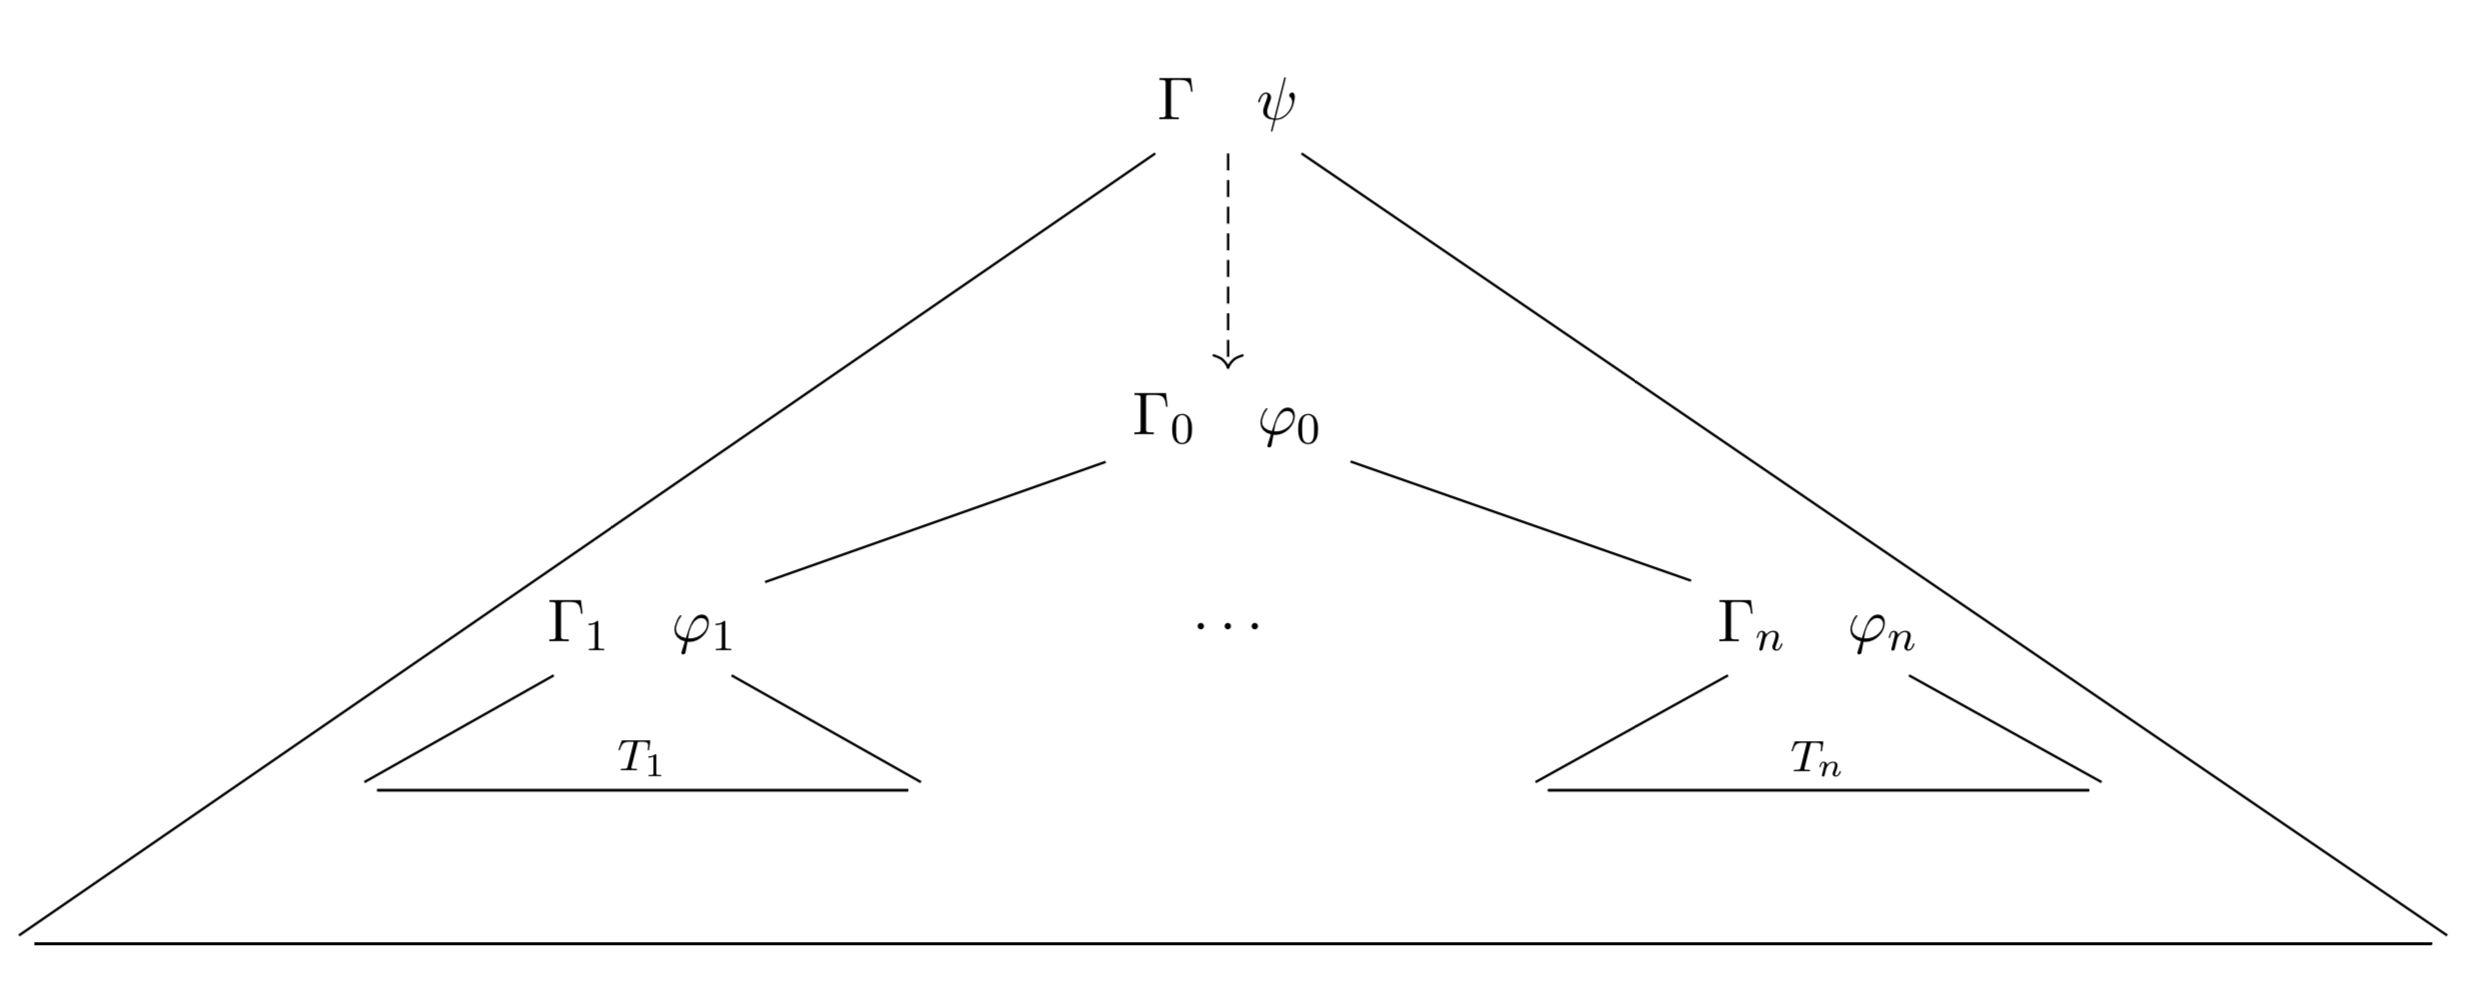
\includegraphics[scale = 0.3]{figures/arbol1.png}
% https://tikzcd.yichuanshen.de/#N4Igdg9gJgpgziAXAbVABwnAlgFyxMJZAVgBoAGAXVJADcBDAGwFcYkQAdDgcXoFs+9AARcsUenAAWIjmmwgAvqXSZc+QijIAmanSat2XXgPoB9cqPFSuDAE5pJWc4uUgM2PASIBmUt90MLGyInDz8gqYAjJYSkjb09o5RLioe6kQA7H4B+sGhxhFgMdYcdg5OhEqpal6a2TSBBiFcAMZQEDgIVW6qnhrIWqQALDlB7Ck9abXIQ8OjTSAT7jX9AGxzDbnj3ct9RAAcG3pjIUu96SjkpMTzeWdT-ZFXN5sniwq6MFAA5vBEoAAzWwQPhISI0HAQJBabpAkFgiFQxDeWHA0GIQYgSFIMggSQwehQdiQMBsVHwjGIpDrPEEokhElk1xw9G47GIGmMLCk9hwCBcok0fGE4kENgQ+hYRiink0Rj0ABGMEYAAVzrUQLYsN9JDgQDQpFgAXrEABaFHMtHUqmIXHC+ngMX6kCG41IXwgeVK1XqjSa7W652NPIAFWS5PRHvZWVpIoZToj7pth1jDsZExZSBj7JT9pl4pdjjdZotgKtiBT0aFdPzztdJo9XuVaoe7C1Or1rwWYcqlopVyxSPBICVYHpA65PJCVnxRMTiAH7IAnNW446efPF0OB3n4xu++iV4OwTua3uC-WkOb508bUfd+uL0WGx8FEA
\begin{comment}
\begin{tikzcd}
                               &  &                        &                                                                 &                                & \Gamma \quad \psi \arrow[dd, dashed] \arrow[lllllddddd, no head] \arrow[rrrrrddddd, no head] &                        &                                                                 &                                &  &                                \\
                               &  &                        &                                                                 &                                &                                                                                               &                        &                                                                 &                                &  &                                \\
                               &  &                        &                                                                 &                                & \Gamma_0\quad\varphi_0 \arrow[lld] \arrow[rrd]                                               &                        &                                                                 &                                &  &                                \\
                               &  &                        & \Gamma_1\quad\varphi_1 \arrow[ld, no head] \arrow[rd, no head] &                                & \cdots                                                                                        &                        & \Gamma_n\quad\varphi_n \arrow[ld, no head] \arrow[rd, no head] &                                &  &                                \\
                               &  & {} \arrow[rr, no head] &                                                                 & {} \arrow[ll, "A_1"', no head] &                                                                                               & {} \arrow[rr, no head] &                                                                 & {} \arrow[ll, "A_n"', no head] &  &                                \\
{} \arrow[rrrrrrrrrr, no head] &  &                        &                                                                 &                                &                                                                                               &                        &                                                                 &                                &  & {} \arrow[llllllllll, no head]
\end{tikzcd}
\end{comment}
\end{center}
donde $T_i$ es el árbol de deducción que se ha usado para llegar a $\Gamma_i\idash\varphi_i$. Ahora, simplemente, cambiamos el grafo formado por el nodo y sus $n$ hijos por el árbol de deducción de la regla derivada. Cuando en una hoja del árbol de la regla derivada aparece una secuencia $\Gamma_i\idash\varphi_i$, añadimos debajo de ella el árbol de deducción $T_i$. De modo que esquemáticamente obtenemos un árbol así:

\begin{center}
\begin{comment}
% https://tikzcd.yichuanshen.de/#N4Igdg9gJgpgziAXAbVABwnAlgFyxMJZAVgBoAGAXVJADcBDAGwFcYkQAdDgcXoFs+9AARcsUenAAWIjmmwgAvqXSZc+QijIAmanSat2XXgPoB9cqPFSuDAE5pJWc4uUgM2PASIBmUt90MLGyInDz8gqZYXACOzPRQNvT2jpEuKh7qRADsfgH6waHGEQBWMXEJHHYOTsVpbqqeGshapAAseUHsde5qXiitbR0GId0NmSgAbIM0gcMgoxl9yAAc03qdI0rpvU3kpMRDBQs7RACMewcz+V1b9YtNZP5XGyAAggAe+IIICrowUABzeBEUAAM1sED4SFONBwECQLRAkhg8XYkDAbBoUiwoJw0Nu4Mh0Nh8MQviRKKgaIImJA2NxSAAtKcCRCoYhEXCkAMKaiQui2KyiRySUgyLyqfyaXVCeyeVzEOLGFgMew4BBlVSaMi+eBpbD6FhGNTVTRGPQAEYwRgABTGfRAtiwAMkeKxjgZiHIQvZ4oVPJ1kr1prpHrxXrNlutdvu7CdLrd6zmABVUj6kOSFVMJSbacrVSF1ZqQAajbmSyBzVbbfaNI7na6ZWyM6LEDkc1LVenENmFe3A+X3Tjw97XLKkO2s9rKYPQ8OkHtK1Ga7GQvHG88U6Zat3FwqYSArWBJYv8wUrMiqbvW6sO8HBWPmxGQAqAJzT3UCpvC29vj9Br8h09UcwSfd8X1JW8B07Wl6RHbtOVJcloPvCs4KZbxu0zUlEXQsl-1nWYCmTCsq2jWs4wbPFfgUIA
\begin{tikzcd}
                               &  &                        &                                                                                                    &                                & \Gamma \idash \psi \arrow[dd, dashed] \arrow[lllllddddd, no head] \arrow[rrrrrddddd, no head] &                        &                                                                                                           &                                &  &                                \\
                               &  &                        &                                                                                                    &                                &                                                                                               &                        &                                                                                                           &                                &  &                                \\
                               &  &                        &                                                                                                    &                                & \Gamma_0\idash\varphi_0 \arrow[lld, no head, shift right] \arrow[rrd, no head, shift left]    &                        &                                                                                                           &                                &  &                                \\
                               &  &                        & \Gamma_i\quad\varphi_i \arrow[ld, no head] \arrow[rd, no head] \arrow[rrrr, no head, shift left=3] &                                & Axiomas                                                                                       &                       & \Gamma_j\quad\varphi_j \arrow[ld, no head] \arrow[rd, no head] \arrow[llll, "T"', no head, shift right=3] &                                &  &                                \\
                               &  & {} \arrow[rr, no head] &                                                                                                    & {} \arrow[ll, "T_i"', no head] &                                                                                               & {} \arrow[rr, no head] &                                                                                                           & {} \arrow[ll, "T_j"', no head] &  &                                \\
{} \arrow[rrrrrrrrrr, no head] &  &                        &                                                                                                    &                                &                                                                                               &                        &                                                                                                           &                                &  & {} \arrow[llllllllll, no head]
\end{tikzcd}
\end{comment}
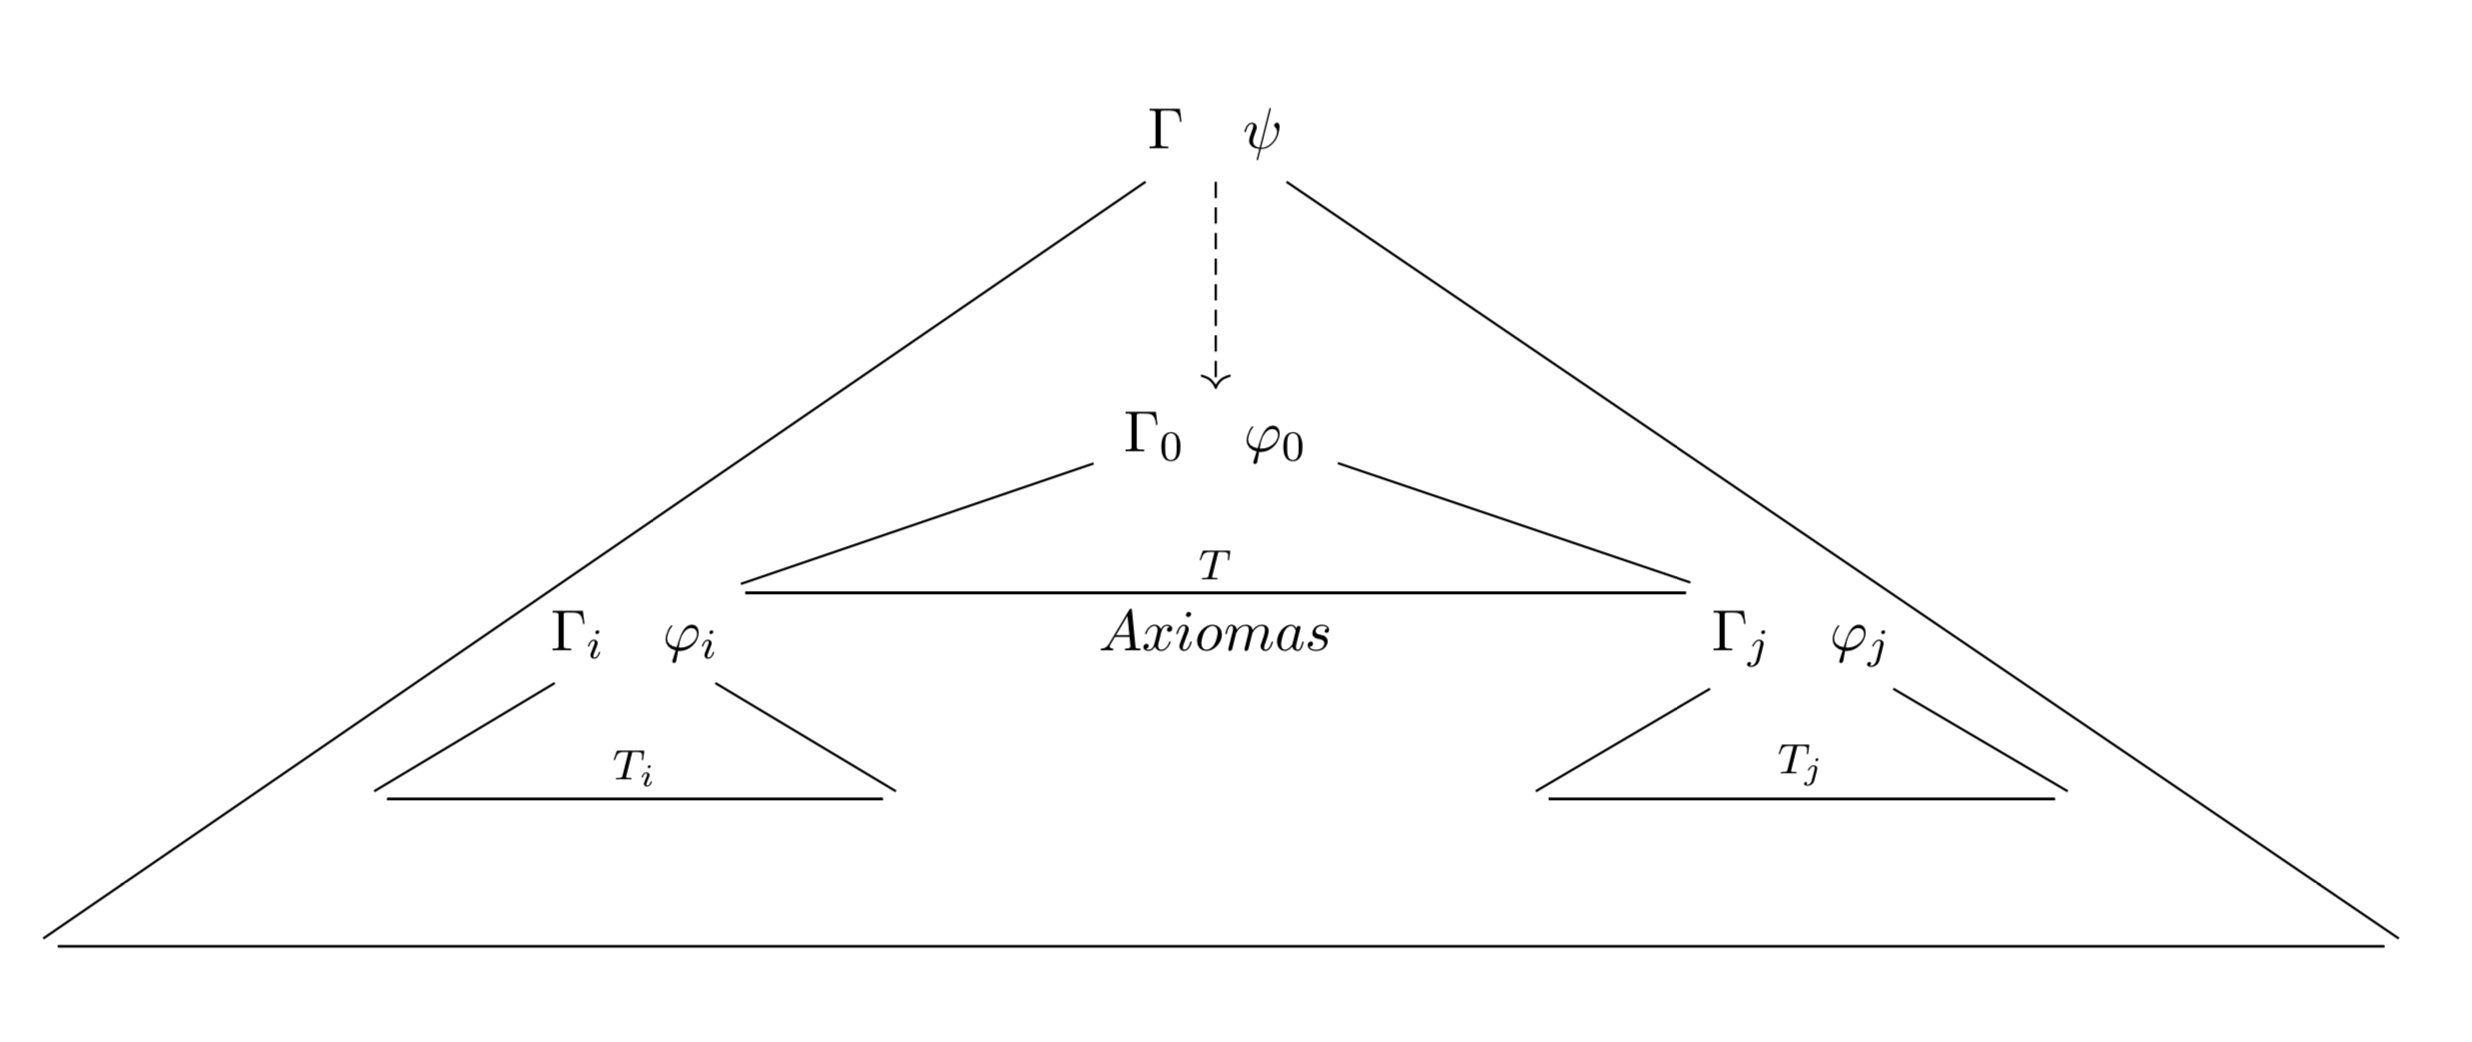
\includegraphics[scale = 0.3]{figures/arbol2.png}
\end{center}
donde en el árbol $T$ solo se usan reglas básicas y axiomas. Se puede demostrar que sustituyendo de este modo todas las reglas derivadas acabamos obteniendo un árbol en el que solo hay reglas básicas y axiomas.\\[10pt]
De modo que por lo que acabamos de ver, si tenemos un árbol para $\Gamma\idash\varphi$ que usa reglas básicas y derivadas, se cumple que $\Gamma\idash\varphi$ es formalmente deducible. Esto quiere decir que podemos usar sin problemas reglas derivadas que conocemos en los árboles de deducción.

\subsection{Repertorio de reglas derivadas}
En esta sección expondremos muchas reglas derivadas que permiten ver cómo razonamientos que hacemos habitualmente se expresan en el cálculo de secuencias. Para casi todas las reglas derivadas incluímos sus árboles de deducción.

\begin{itemize}
    \item Eliminación de una conjunción: \emph{siempre podemos demostrar un resultado más fuerte}. Son dos reglas simétricas.
    \begin{center}
      \centerAlignProof
       ($\textbf{E} \land$)
      \quad
      \centerAlignProof
        \AxiomC{$\Gamma \idash \psi\land\varphi$}
        \UnaryInfC{$\Gamma \idash \varphi $}
      \DisplayProof
      \qquad
      \centerAlignProof
        \AxiomC{$\Gamma \idash \varphi\land\psi$}
        \UnaryInfC{$\Gamma \idash \varphi $}
      \DisplayProof
    \end{center}
    \begin{proof} \mbox{}
          \begin{center}
            \begin{tikzpicture}[sibling distance=5cm]
          \node (1) {\(\Gamma\idash \varphi\)}
              child{
                node (2){\(\Gamma\idash \psi\land\varphi\)}
              }
              child{
                node{\(\Gamma,\psi\land\varphi\idash \varphi\)}
                child{
                  node (3){\(\Gamma,\psi,\varphi\idash \varphi\)}
                  edge from parent node [right]{\(\regla{\land A}\)}
                }
              };
              \node[below=0mm of 1] {\(\regla{RC}\)};
              \node[below=0mm of 2] {Premisa};
              \node[below=0mm of 3] {\(\regla{SP}\)};
            \end{tikzpicture}
          \end{center}
    \end{proof}
    
    \item Modus Ponens
    \begin{center} 
      \centerAlignProof
       ($\textbf{MP}$)
      \quad
      \centerAlignProof
        \AxiomC{$\Gamma \idash \varphi \qquad \Gamma \idash \varphi \rightarrow \psi$}
        \UnaryInfC{$\Gamma \idash \psi $}
      \DisplayProof
    \end{center}
    \begin{proof} \mbox{}
        \begin{center}
    \begin{tikzpicture}[sibling distance=5cm]
      \node (1){\(\Gamma\idash \psi\)}
      child{
        node (2){\(\Gamma\idash \varphi\)}
      }
      child{
        node (3){\(\Gamma,\varphi\idash \psi\)}
        child{
          node (4){\(\Gamma,\varphi,\varphi\rightarrow\psi\idash\psi\)}
          child{
            node
            (6){\(\Gamma,\varphi,\varphi\rightarrow\psi\idash\varphi\)}
          }
          child{node (7){\(\Gamma,\psi\idash\psi\)}}
        }
        child{
          node {\(\Gamma,\varphi\idash\varphi\rightarrow\psi\)}
          child{
            node(5){\(\Gamma\idash\varphi\rightarrow\psi\)}
            edge from parent node[right]{\(\regla{FS}\)}
          }
        }
      };
      \node[below=0mm of 1] {\(\regla{RC}\)};
      \node[below=0mm of 2] {Premisa};
      \node[below=0mm of 3] {\(\regla{RC}\)};
      \node[below=0mm of 4] {\(\regla{\rightarrow A}\)};
      \node[below=0mm of 5] {Premisa};
      \node[below=0mm of 6] {SP};
      \node[below=0mm of 7] {SP};

    \end{tikzpicture}
  \end{center}
    \end{proof}
    \item Variante de la conjunción en el consecuente.
    \begin{center} 
      \centerAlignProof
       ($\land \textbf{C}'$)
      \quad
      \centerAlignProof
        \AxiomC{}
        \UnaryInfC{$\Gamma, \varphi, \psi \idash \varphi\land\psi $}
      \DisplayProof
    \end{center}
    \begin{proof} \mbox{}
         \begin{center}
            \begin{tikzpicture}[sibling distance=5cm]
              \node (1){\(\Gamma,\varphi,\psi\idash \varphi\land\psi\)}
              child{
                node (2) {\(\Gamma,\varphi,\psi\idash \varphi\)}
              }
              child{
                node (3) {\(\Gamma,\varphi,\psi\idash \psi\)}
              };
              \node[below=0mm of 1]{\(\regla{\land C}\)};
              \node[below=0mm of 2]{\(\regla{SP}\)};
              \node[below=0mm of 3]{\(\regla{SP}\)};
            \end{tikzpicture}
          \end{center}
    \end{proof}
    
    \item Variante de la disyunción en el consecuente.
    \begin{center} 
      \centerAlignProof
       ($\lor \textbf{C}'$)
      \quad
      \centerAlignProof
        \AxiomC{}
        \UnaryInfC{$\Gamma, \varphi \idash \varphi\lor\psi $}
      \DisplayProof
      \quad
      \centerAlignProof
        \AxiomC{}
        \UnaryInfC{$\Gamma, \psi \idash \varphi\lor\psi $}
      \DisplayProof
    \end{center}
    \begin{proof} \mbox{}
         \begin{center}
            \begin{tikzpicture}
              \node{\(\Gamma,\varphi\idash \varphi\lor\psi\)}
              child{
                node(1){\(\Gamma,\varphi\idash \varphi\)}
                edge from parent node[right]{\(\regla{\lor C}\)}
              }
              ;
              \node[below=0mm of 1]{\(\regla{SP}\)};
            \end{tikzpicture}
          \end{center}
    \end{proof}
    
    \item Reducción al absurdo: \emph{suponer la negación de la conclusión y llegar a una contradicción}.
    \begin{center} 
      \centerAlignProof
       ($\textbf{RA}!$)
      \quad
      \centerAlignProof
        \AxiomC{$\Gamma,\neg \varphi \idash \bot$}
        \UnaryInfC{$\Gamma \idash \varphi $}
      \DisplayProof
    \end{center}
    \begin{proof} \mbox{}
        \begin{center}
        \begin{tikzpicture}
          \node{\(\Gamma\idash \varphi\)}
            child{
              node{\(\Gamma\idash \neg\neg\varphi\)}
              child{
                node (1){\(\Gamma,\neg\varphi\idash\bot\)}
                edge from parent node[right]{\(\regla{\neg C}\)}
              }
              edge from parent node[right]{\(\regla{DN!}\)}
            }
            ;
            \node[below=0mm of 1]{Premisa};
        \end{tikzpicture}
      \end{center}
    \end{proof}
    
    \item Reglas de la contradicción.
    \begin{center} 
      \centerAlignProof
       ($\textbf{CT}_1$)
      \quad
      \centerAlignProof
        \AxiomC{$\Gamma \idash \psi \qquad \Gamma \idash \neg\psi$}
        \UnaryInfC{$\Gamma \idash \varphi $}
      \DisplayProof
    \end{center}
    
    \begin{proof} \mbox{}
        \begin{center}
        \begin{tikzpicture}[sibling distance=5cm]
          \node(0){\(\Gamma\idash \varphi\)}
            child{
              node(1){$\Gamma, \bot \idash \varphi$}
            }
            child{
              node(2){$\Gamma \idash \bot$}
              child{
                  node(3){$\Gamma, \neg \psi \idash \bot$}
                  child {
                        node(5){$\Gamma, \neg \psi \idash \psi$}
                        child {
                            node(6){$\Gamma\idash \psi$}
                            edge from parent node[right]{\(\regla{FS}\)}
                        }
                        edge from parent node[right]{\(\regla{\neg A}\)}
                  }
              }
              child{
                  node(4){$\Gamma \idash \neg \psi$}
              }
            }
            ;
            \node[below=0mm of 0]{(\textbf{RC})};
            \node[below=0mm of 1]{($\bot$ \textbf{A})};
            \node[below=0mm of 2]{(\textbf{RC})};
            \node[below=0mm of 4]{Premisa};
            \node[below=0mm of 6]{Premisa};
        \end{tikzpicture}
      \end{center}
    \end{proof}
    
    \begin{center} 
      \centerAlignProof
       ($\textbf{CT}_2$)
      \quad
      \centerAlignProof
        \AxiomC{}
        \UnaryInfC{$\Gamma, \varphi, \neg\varphi \idash \psi $}
      \DisplayProof
    \end{center}
    
        \begin{proof} \mbox{}
        \begin{center}
        \begin{tikzpicture}[sibling distance=4cm]
            \node(0){$\Gamma, \varphi, \neg\varphi \idash \psi$}
            child {
                node(1){$\Gamma, \varphi, \neg \varphi, \idash \neg \varphi$}
            }
            child {
                node(2){$\Gamma, \varphi, \neg \varphi, \idash \varphi$}
            }
            ;
            \node[below=0mm of 0]{($\textbf{CT}_1$)};
            \node[below=0mm of 1]{(\textbf{SP})};
            \node[below=0mm of 2]{(\textbf{SP})};
        \end{tikzpicture}
      \end{center}
      
      
    \end{proof}
    \item  Reglas de la doble negación.
    
    \begin{center} 
      \centerAlignProof
       ($\neg\neg\textbf{C}$)
      \quad
      \centerAlignProof
        \AxiomC{$\Gamma \idash \varphi$}
        \UnaryInfC{$\Gamma \idash \neg\neg\varphi $}
      \DisplayProof
      \qquad 
      \centerAlignProof
       ($\neg\neg\textbf{A}!$)
      \quad
      \centerAlignProof
        \AxiomC{$\Gamma,\varphi\idash \psi$}
        \UnaryInfC{$\Gamma,\neg\neg\varphi\idash \psi$}
      \DisplayProof
    \end{center}
    
    \begin{proof} \mbox{}
        \begin{center}
        \begin{tikzpicture}[sibling distance=4cm]
            \node(0){$\Gamma \idash \neg\neg\varphi$}
            child{
                node(1){$\Gamma\idash \varphi$}
            }
            child {
                node(2){$\Gamma,\varphi \idash \neg\neg \varphi$}
                child {
                    node(3) {$\Gamma,\varphi,\neg\varphi \idash \bot$}
                    edge from parent node[right]{\(\regla{\neg C}\)}
                }
            }
            ;
            \node[below=0mm of 0]{($\textbf{RC}$)};
            \node[below=0mm of 1]{Premisa};
            \node[below=0mm of 3]{($\textbf{CT}_2$)};
        \end{tikzpicture}
        \end{center}
        \begin{center}
        \begin{tikzpicture}[sibling distance=4cm]
            \node(0){$\Gamma,\neg\neg\varphi\idash \psi$}
            child{
                node(1){$\Gamma,\neg\neg\varphi\idash \varphi$}
                child {
                    node(3){$\Gamma,\neg\neg\varphi \idash \neg\neg\varphi$}
                    edge from parent node[right]{\(\regla{DN!}\)}
                }
            }
            child {
                node(2){$\Gamma,\neg\neg\varphi,\varphi \idash \psi$}
                child {
                    node(4){$\Gamma,\varphi \idash \psi$}
                    edge from parent node[right]{\(\regla{FS}\)}
                }
            }
            ;
            \node[below=0mm of 0]{($\textbf{RC}$)};
            \node[below=0mm of 3]{($\textbf{SP}$)};
            \node[below=0mm of 4]{Premisa};
        \end{tikzpicture}
      \end{center}
      
    \end{proof}
    
    \item  Reglas de la contraposición.
    
    \begin{center} 
      \centerAlignProof
       ($\textbf{CP}_1$)
      \quad
      \centerAlignProof
        \AxiomC{$\Gamma,\psi \idash \varphi$}
        \UnaryInfC{$\Gamma,\neg \varphi \idash \neg\psi $}
      \DisplayProof
      \qquad 
      \centerAlignProof
       ($\textbf{CP}_2$)
      \quad
      \centerAlignProof
        \AxiomC{$\Gamma,\varphi \idash \neg\psi $}
        \UnaryInfC{$\Gamma,\psi \idash \neg\varphi$}
      \DisplayProof
    \end{center}
    
    \begin{proof} \mbox{}
        \begin{center}
        \begin{tikzpicture}[sibling distance=4cm]
            \node(0) {$\Gamma,\neg\varphi \idash \neg\psi$}
            child {
                node(1){$\Gamma, \neg\varphi, \psi \idash \bot$}
                child {
                    node(2){$\Gamma, \neg\varphi, \psi \idash \varphi$}
                    child {
                        node(4){$\Gamma, \psi \idash \varphi$}
                        edge from parent node[right]{($\textbf{FS}$)}
                    }
                }
                child {
                    node(3){$\Gamma, \neg\varphi, \psi, \varphi \idash \bot$}
                }
                edge from parent node[right]{($\neg\textbf{C}$)}
            }
            ;
             \node[below=0mm of 1]{($\textbf{RC}$)};
             \node[below=0mm of 3]{($\textbf{CT}_2$)};
             \node[below=0mm of 4]{Premisa};
        \end{tikzpicture}
        \end{center}
        
    \end{proof}
    
    \begin{center} 
      \centerAlignProof
       ($\textbf{CP}_3!$)
      \quad
      \centerAlignProof
        \AxiomC{$\Gamma,\neg\varphi \idash \neg\psi$}
        \UnaryInfC{$\Gamma,\psi \idash \varphi $}
      \DisplayProof
      \qquad 
      \centerAlignProof
       ($\textbf{CP}_4!$)
      \quad
      \centerAlignProof
        \AxiomC{$\Gamma,\neg\varphi \idash \psi$}
        \UnaryInfC{$\Gamma,\neg\psi \idash \varphi $}
      \DisplayProof
    \end{center}
    \begin{proof} \mbox{}
        \begin{center}
        \begin{tikzpicture}[sibling distance=4cm]
            \node(0) {$\Gamma,\psi \idash \varphi$}
            child {
                node(1){$\Gamma, \psi \idash \neg\neg\varphi$}
                child {
                    node(2){$\Gamma, \neg\varphi \idash \neg\psi$}
                    edge from parent node[right]{($\textbf{CP}_2$)}
                }
                edge from parent node[right]{($\textbf{DN}!$)}
            }
            ;
            \node[below=0mm of 2]{Premisa};
        \end{tikzpicture}
        \end{center}
        
    \end{proof}
    
    \item  Otras reglas no constructivas.
    
    \begin{center} 
      \centerAlignProof
       ($\textbf{VC}!$)
      \quad
      \centerAlignProof
        \AxiomC{$\Gamma,\neg\varphi \idash \psi$}
        \UnaryInfC{$\Gamma\idash \varphi \lor\psi $}
      \DisplayProof
      \qquad 
      \centerAlignProof
        \AxiomC{$\Gamma,\neg\psi \idash \varphi$}
        \UnaryInfC{$\Gamma\idash \varphi \lor\psi $}
      \DisplayProof
    \end{center}
    
    \begin{proof} \mbox{}
        \begin{center}
        \begin{tikzpicture}[sibling distance=4cm]
            \node(0) {$\Gamma\idash \varphi \lor\psi$}
            child {
                node(1) {$\Gamma, \neg(\varphi\lor \psi)\idash \bot$}
                child {
                    node(2) {$\Gamma, \neg(\varphi\lor \psi)\idash \varphi\lor \psi$}
                    child {
                        node(3) {$\Gamma, \neg(\varphi\lor \psi)\idash \varphi$}
                        child {
                            node(4) {$\Gamma, \neg \varphi \idash \varphi\lor\psi$}
                            child {
                                node(5){$\Gamma, \neg\varphi\idash \psi$}
                                edge from parent node [right]{($\lor\textbf{C}$)}
                            }
                            edge from parent node [right]{($\textbf{CP}_4$)}
                        }
                        edge from parent node[right]{($\lor\textbf{C}$)}
                    }
                    edge from parent node[right]{($\neg\textbf{A}$)}
                }
                edge from parent node[right]{($\textbf{RA}!$)}
            }
            
            ;
            \node[below=0mm of 5]{Premisa};
        \end{tikzpicture}
        \end{center}
    \end{proof}
    
    \begin{center} 
      \centerAlignProof
       ($\textbf{TE}!$)
      \quad
      \centerAlignProof
        Tercio excluido
      \qquad 
      \centerAlignProof
        \AxiomC{}
        \UnaryInfC{$\Gamma\idash \varphi \lor\neg\varphi $}
      \DisplayProof
    \end{center}
     \begin{proof} \mbox{}
        \begin{center}
        \begin{tikzpicture}[sibling distance=4cm]
            \node(0) {$\Gamma\idash \varphi \lor\neg\varphi$}
            child {
                node(1) {$\Gamma, \neg\varphi \idash \neg\varphi$}
                edge from parent node[right]{($\lor\textbf{C}!$)}
            }
            
            ;
            \node[below=0mm of 1]{($\textbf{SP}$)};
        \end{tikzpicture}
        \end{center}
    \end{proof}
    
    \begin{center} 
      \centerAlignProof
       ($\textbf{DC}!$)
      \quad
      \centerAlignProof
        Distinción de casos
      \qquad 
      \centerAlignProof
        \AxiomC{$\Gamma, \varphi\idash \psi\qquad \Gamma, \neg\varphi\idash \psi$}
        \UnaryInfC{$\Gamma\idash \psi$}
      \DisplayProof
    \end{center}
    \begin{proof} \mbox{}
        \begin{center}
        \begin{tikzpicture}[sibling distance=4cm]
            \node(0) {$\Gamma\idash \psi$}
            child {
                node(1) {$\Gamma \idash \varphi\lor\neg\varphi$}
            }
            child {
                node(2) {$\Gamma,\varphi\lor\neg\varphi \idash \psi$}
                child {
                    node(3) {$\Gamma, \varphi \idash \psi$}
                }
                child {
                    node(4) {$\Gamma, \neg\varphi \idash \psi$}
                }
            }
            ;
            \node[below=0mm of 0]{($\textbf{RC}$)};
            \node[below=0mm of 1]{($\textbf{TE}$!)};
            \node[below=0mm of 2]{($\lor\textbf{A}$!)};
            \node[below=0mm of 3]{Premisa};
            \node[below=0mm of 4]{Premisa};
        \end{tikzpicture}
        \end{center}
    \end{proof}
    
    \begin{center} 
      \centerAlignProof
       ($\rightarrow\textbf{A}!$)
      \quad
      \qquad 
      \centerAlignProof
        \AxiomC{$\Gamma, \neg \varphi  \idash \chi \qquad \Gamma, \psi  \idash \chi$}
        \UnaryInfC{$\Gamma, \varphi \rightarrow \psi \idash \chi$}
      \DisplayProof
    \end{center}
    \begin{proof} \mbox{}
        \begin{center}
            \begin{tikzpicture}[sibling distance=5cm]
                \node(0) {$\Gamma, \varphi \rightarrow \psi \idash \chi$}
                child {
                    node(1) {$\Gamma, \neg \varphi, \varphi \rightarrow\psi \idash \chi$}
                    child {
                        node(3) {$\Gamma, \neg \varphi \idash \chi$}
                        edge from parent node[right]{($\textbf{FS}$)}
                    }
                }
                child {
                    node(2) {$\Gamma, \varphi, \varphi \rightarrow\psi \idash \chi$}
                    child {
                        node(4) {$\Gamma, \varphi, \varphi\rightarrow \psi \idash \varphi$}
                    }
                    child {
                        node(5) {$\Gamma, \varphi, \psi \idash \chi$}
                        child {
                            node(6){$\Gamma,\psi \idash \chi$}
                            edge from parent node[right]{($\textbf{FS}$)}
                        }
                    }
                }
                ;
                \node[below=0mm of 0]{($\textbf{DC}$!)};
                \node[below=0mm of 2]{($\rightarrow\textbf{A}$)};
                \node[below=0mm of 3]{Premisa};
                \node[below=0mm of 4]{($\textbf{SP}$)};
                \node[below=0mm of 6]{Premisa};
            \end{tikzpicture}
        \end{center}
    \end{proof}
    

    
    \begin{center} 
      \centerAlignProof
       ($\neg\rightarrow\textbf{A}!$)
      \quad
      \centerAlignProof
        \AxiomC{$\Gamma,\varphi, \neg \psi \idash \chi$}
        \UnaryInfC{$\Gamma, \neg(\varphi \rightarrow \psi)\idash \chi$}
      \DisplayProof
    \end{center}
    \begin{proof} \mbox{}
        \begin{center}
            \begin{tikzpicture}[sibling distance=5cm]
                \node(0) {$\Gamma, \neg(\varphi \rightarrow \psi)\idash \chi$}
                child {
                    node(1){$\Gamma,\neg \chi\idash \varphi\rightarrow\psi$}
                    child {
                        node(2){$\Gamma,\neg \chi, \varphi\idash \psi$}
                        child {
                            node(3){$\Gamma,\varphi, \neg \psi\idash \chi$}
                            edge from parent node[right]{$(\textbf{CP}_4!)$}
                        }
                        edge from parent node[right]{$(\rightarrow\textbf{C})$}
                    }
                    edge from parent node[right]{$(\textbf{CP}_4!)$}
                }
                ;
                \node[below=0mm of 3]{$Premisa$};
            \end{tikzpicture}
        \end{center}
    \end{proof}
    \item Leyes de De Morgan.
    
    \begin{center} 
      \centerAlignProof
       ($\textbf{DM}_1$)
      \quad
      \centerAlignProof
        \AxiomC{$\idash$}
        \UnaryInfC{$\Gamma, \neg \varphi \lor \neg \psi\idash \neg(\varphi \land \psi)$}
      \DisplayProof
    \end{center}
    \begin{proof} \mbox{}
        \begin{center}
            \begin{tikzpicture}[sibling distance=5cm]
            \node(0) {$\Gamma, \neg\varphi\lor\neg\psi\idash \neg(\varphi\land\psi)$}
            child {
                node(1){$\Gamma, \varphi\land\psi\idash \neg(\neg\varphi\lor\neg\psi)$}
                child {
                    node(2){$\Gamma, \varphi, \psi\idash \neg(\neg\varphi\lor \neg\psi)$}
                    child {
                        node(4){$\Gamma, \varphi, \psi, \neg\varphi\lor \neg\varphi \idash \bot$}
                        child {
                            node(5) {$\Gamma, \varphi, \psi, \neg\varphi\idash \bot$}
                        }
                        child {
                            node(6) {$\Gamma, \varphi, \psi, \neg\psi\idash \bot$}
                        }
                        edge from parent node[right]{$(\neg\textbf{C})$}
                    }
                    edge from parent node[right]{$(\land\textbf{A})$}
                }
                edge from parent node[right]{$(\textbf{CP}_2)$}
            }
            ;
            \node[below=0mm of 4]{($\lor\textbf{A}$)};
            \node[below=0mm of 5]{($\textbf{CT}_2$)};
            \node[below=0mm of 6]{($\textbf{CT}_2$)};
        \end{tikzpicture}
        \end{center}
        
        
        
        
    \end{proof}
    \begin{center}
        \centerAlignProof
       ($\textbf{DM}_2$)
      \quad
      \centerAlignProof
        \AxiomC{$\idash$}
        \UnaryInfC{$\Gamma, \neg (\varphi \land \psi) \idash \neg \varphi \lor \neg \psi$}
      \DisplayProof
    \end{center}
    \begin{proof}\mbox{}
    \begin{center}

    \begin{tikzpicture}[sibling distance=5cm]
            \node(0) {$\Gamma, \neg(\varphi\land \psi)\idash \neg\varphi\lor \neg \psi$}
            child {
                node(1) {$\Gamma, \neg(\neg\varphi\lor\neg\psi)\idash \varphi\land\psi$}
                child {
                    node(2) {$\Gamma, \neg(\neg\varphi\lor\neg\psi)\idash \varphi$}
                    child {
                        node(4) {$\Gamma, \neg \varphi \idash \neg\varphi\lor \neg\psi$}
                        child {
                            node(5) {$\Gamma, \neg \varphi \idash \neg\varphi$}
                            edge from parent node[right]{$(\lor\textbf{C})$}
                        }
                        edge from parent node[right]{$(\textbf{CP}_4!)$}
                    }
                }
                child {
                    node(3) {$\Gamma, \neg(\neg\varphi\lor\neg\psi)\idash \psi$}
                    child {
                        node(6) {$\Gamma, \neg \psi \idash \neg\varphi\lor \neg\psi$}
                        child {
                            node(7) {$\Gamma, \neg \varphi \idash \neg\psi$}
                            edge from parent node[right]{$(\lor\textbf{C})$}
                        }
                        edge from parent node[right]{$(\textbf{CP}_4!)$}
                    }
                }
                edge from parent node[right]{$(\textbf{CP}_4)$}
            }
            ;
            \node[below=0mm of 1]{($\land\textbf{C}$)};
            \node[below=0mm of 5]{($\textbf{SP}$)};
            \node[below=0mm of 7]{($\textbf{SP}$)};
    \end{tikzpicture}
    
    
\end{center}
    \end{proof}
    \begin{center} 
      \centerAlignProof
       ($\textbf{DM}_3$)
      \quad
      \centerAlignProof
        \AxiomC{$\idash$}
        \UnaryInfC{$\Gamma, \neg \varphi \land \neg \psi \idash \neg (\varphi \lor \psi)$}
      \DisplayProof
    \end{center}
    
    \begin{center}
      \centerAlignProof
       ($\textbf{DM}_4$)
      \quad
      \centerAlignProof
        \AxiomC{$\idash$}
        \UnaryInfC{$\Gamma, \neg (\varphi \lor \psi) \idash \neg \varphi \land \neg \psi$}
      \DisplayProof
    \end{center}
    \item Ley de Pierce
    \begin{center} 
      \centerAlignProof
       
      \quad
      \centerAlignProof
        \AxiomC{$\idash$}
        \UnaryInfC{$\Gamma\idash ((\varphi\rightarrow \psi)\rightarrow\varphi)\rightarrow \varphi$}
      \DisplayProof
    \end{center}
    \item Reglas de ejemplificación. ($t\in TERM_{\overline{S}}$)
    \begin{center} 
      \centerAlignProof
       ($\textbf{E}\forall_1$)
      \quad
      \centerAlignProof
        \AxiomC{$\idash$}
        \UnaryInfC{$\Gamma, \forall x\ \varphi \idash \varphi[t/x]$}
      \DisplayProof
      \qquad
      \centerAlignProof
       ($\textbf{E}\forall_2$)
      \quad
      \centerAlignProof
        \AxiomC{$\Gamma \idash \forall x\ \varphi$}
        \UnaryInfC{$\Gamma \idash \varphi[t/x]$}
      \DisplayProof
    \end{center}
    \begin{center} 
      \centerAlignProof
       ($\textbf{E}\forall_3$)
      \quad
      \centerAlignProof
        \AxiomC{$\Gamma, \varphi[t/x] \idash \psi$}
        \UnaryInfC{$\Gamma, \forall x\ \varphi \idash \psi$}
      \DisplayProof
    \end{center}
    \begin{proof} \mbox{}
    \begin{center}
    \begin{tikzpicture}[sibling distance=5cm]
            \node(0) {$\Gamma, \forall x \varphi\idash \varphi[t/x]$}
            child {
                node(1) {$\Gamma, \varphi, \varphi[t/x] \idash \varphi[t/x]$}
                edge from parent node[right] {$(\forall \textbf{A})$}
            }
            ;
            \node[below=0mm of 1]{($\textbf{SP}$)};
    \end{tikzpicture}
    \end{center}
    \begin{center}
    \begin{tikzpicture}[sibling distance=5cm]
            \node(0) {$\Gamma \idash \varphi[t/x]$}
            child {
                node(1) {$\Gamma \forall x\varphi$}
            }
            child {
                node(2) {$\Gamma, \forall x \varphi \idash \varphi[t/x]$}
            }
            ;
            \node[below=0mm of 0]{($\textbf{RC}$)};
            \node[below=0mm of 1]{Premisa};
            \node[below=0mm of 2]{$(\textbf{E}\forall_1)$};
    \end{tikzpicture}
    \end{center}
    \begin{center}
    \begin{tikzpicture}[sibling distance=5cm]
            \node(0) {$\Gamma, \forall x \varphi \idash \psi$}
            child {
                node(1) {$\Gamma, \forall x \varphi \idash \varphi[t/x]$}
            }
            child {
                node(2) {$\Gamma, \forall x \varphi, \varphi[t/x]\idash \psi$}
                child {
                    node(3) {$\Gamma, \varphi[t/x]\idash \psi$}
                    edge from parent node[right]{$(\textbf{RS})$}
                }
            }
            ;
            \node[below=0mm of 0]{$(\textbf{RC})$};
            \node[below=0mm of 1]{$(\textbf{E}\forall_1)$};
            \node[below=0mm of 3]{Premisa};

    \end{tikzpicture}
    
    \end{center}
    
    \end{proof}
    
    \begin{center} 
      \centerAlignProof
       ($\textbf{E}\exists_1$)
      \quad
      \centerAlignProof
        \AxiomC{$\idash$}
        \UnaryInfC{$\Gamma, \varphi[t/x] \idash \exists x\ \varphi$}
      \DisplayProof
      \qquad
      \centerAlignProof
       ($\textbf{E}\exists_2$)
      \quad
      \centerAlignProof
        \AxiomC{$\Gamma,  \exists x\ \varphi \idash \psi$}
        \UnaryInfC{$\Gamma, \varphi[t/x]\idash \psi$}
      \DisplayProof
    \end{center}
    \begin{proof} \mbox{}
        \begin{center}
            
        
        \begin{tikzpicture}[sibling distance=5cm]
                \node(0) {$\Gamma, \varphi[t/x] \idash \exists x \varphi$}
                child {
                    node(1) {$\Gamma, \varphi[t/x] \idash \varphi[t/x]$}
                    edge from parent node[right] {$(\exists \textbf{C})$}
                }
                ;
                \node[below=0mm of 1]{($\textbf{SP}$)};
        \end{tikzpicture}
        \end{center}
        \begin{center}
        \begin{tikzpicture}[sibling distance=5cm]
                \node(0) {$\Gamma, \varphi[t/x] \idash \psi$}
                child {
                    node(1) {$\Gamma, \varphi[t/x] \exists x \varphi \idash \psi$}
                    child {
                        node(3) {$\Gamma, \exists x\varphi\idash \psi$}
                        edge from parent node[right]{$(\textbf{FS})$}
                    }
                }
                child {
                    node(2) {$\Gamma, \varphi[t/x]\idash \exists x\varphi$}
                }
                ;
                \node[below=0mm of 0]{($\textbf{RC}$)};
                \node[below=0mm of 2]{($\textbf{E}\exists_1$)};
                \node[below=0mm of 3]{Premisa};
        \end{tikzpicture}

        \end{center}
    \end{proof}
    
    \item Leyes de dualidad.
    
    \begin{center} 
      \centerAlignProof
       ($\textbf{SDM}_1$)
      \quad
      \centerAlignProof
        \AxiomC{$\idash$}
        \UnaryInfC{$\Gamma, \exists x \neg\varphi \idash \neg \forall x\ \varphi$}
      \DisplayProof
      \qquad
      \centerAlignProof
       ($\textbf{SDM}_2$)
      \quad
      \centerAlignProof
        \AxiomC{$\idash$}
        \UnaryInfC{$\Gamma, \neg \forall x\ \varphi  \idash \exists x \neg\varphi$}
      \DisplayProof
    \end{center}
    
    \begin{center} 
      \centerAlignProof
       ($\textbf{SDM}_3$)
      \quad
      \centerAlignProof
        \AxiomC{$\idash$}
        \UnaryInfC{$\Gamma, \forall x \neg\varphi \idash \neg \exists x\ \varphi$}
      \DisplayProof
      \qquad
      \centerAlignProof
       ($\textbf{SDM}_4$)
      \quad
      \centerAlignProof
        \AxiomC{$\idash$}
        \UnaryInfC{$\Gamma, \neg \exists x\ \varphi  \idash \forall x \neg\varphi$}
      \DisplayProof
    \end{center}
       \begin{proof} Se demuestran la segunda y la cuarta.
        \begin{center}
            \begin{tikzpicture}[sibling distance=5cm]
                \node(0) {$\Gamma, \neg \forall x\ \varphi  \idash \exists x \neg\varphi$}
                child {
                    node(1) {$\Gamma, \neg \exists x \neg \varphi \idash \forall x \varphi $}
                    child {
                        node(2) {$\Gamma, \neg\exists x \neg \varphi \idash \varphi[c/x]$}
                        child {
                            node(3) {$\Gamma, \neg\varphi[c/x] \idash \exists x \neg\varphi$}
                            edge from parent node[right] {$(\textbf{CP}_4!)$}
                        }
                        edge from parent node[right] {$(\forall \textbf{C*})$}
                    }
                    edge from parent node[right] {$(\textbf{CP}_4!)$}
                }
                ;
                \node[below=0mm of 3]{($\textbf{E}\exists_1$)};
            \end{tikzpicture}
        \end{center}
        
        \begin{center}
            \begin{tikzpicture}[sibling distance=5cm]
                \node(0) {$\Gamma, \neg \exists x \varphi \idash \forall x \neg \varphi$}
                child {
                    node(1) {$\Gamma, \neg \exists x \varphi \idash \neg \varphi [c/x]$}
                    child {
                        node(2) {$\Gamma,\neg \varphi[c/x] \idash \exists x \varphi$}
                        edge from parent node[right] {$(\textbf{CP}_1!)$}
                    }
                    edge from parent node[right] {$(\forall \textbf{C*})$}
                }
                ;
                \node[below=0mm of 2]{($\textbf{E}\exists_1$)};
            \end{tikzpicture}
        \end{center}
    \end{proof}
    
    \item Sustitución generalizada
    \begin{center} 
      \centerAlignProof
       ($\textbf{SUST}_n$)
      \quad
      \centerAlignProof
        \AxiomC{$\Gamma\idash \varphi[t_1/x_1, ..., t_n/x_n]$}
        \UnaryInfC{$\Gamma, t_1 \doteq s_1, ..., t_n \doteq s_n \idash \varphi[s_1/x_1, ..., s_n/x_n]$}
      \DisplayProof
    \end{center}
    \begin{proof} Por inducción sobre n.
    
    (POR COMPLETAR)
    \end{proof}
\end{itemize}

\section{Ejemplo de uso de deducción natural}
Como ejemplo, intentaremos demostrar que se cumple la siguiente frase:\\

\textit{No existe el barbero que sea el barbero que afeite a los barberos que no se afeitan a sí mismos.}\\

Para formalizar esto, usaremos los predicados $p|_1$ y $a|_2$, donde $p(x)$ significa `$x$ es barbero' y $a(x,y)$ significa `$x$ afeita a $y$'.

Entonces, la conclusión a la que queremos llegar es:

\[\neg\exists x b(x)\land(\forall y b(y)\to(a(x,y)\leftrightarrow \neg a(y,y)))\]

Y no tenemos ninguna premisa. Pasamos directamente al árbol de deducción:

        \begin{center}
            \begin{tikzpicture}[level 1/.style={sibling distance=55mm},level 9/.style={sibling distance=70mm},level 10/.style={sibling distance=35mm}]
]
                \node(0) {$\neg\exists x b(x)\land(\forall y b(y)\to(a(x,y)\leftrightarrow \neg a(y,y)))$}
                child {
                node(1){$\exists x b(x)\land(\forall y b(y)\to(a(x,y)\leftrightarrow \neg a(y,y)))\idash\bot$
                }
                child {
                node(2){$b(c)\land(\forall y b(y)\to(a(c,y)\leftrightarrow \neg a(y,y)))\idash\bot$}
                child{
                node(3){$b(c),\forall y b(y)\to(a(c,y)\leftrightarrow \neg a(y,y))\idash\bot$}
                child{
                node(4){$b(c),\forall y b(y)\to(a(c,y)\leftrightarrow \neg a(y,y)),b(c)\to(a(c,c)\leftrightarrow \neg a(c,c))\idash\bot$}
                child{
                node(5){$b(c),b(c)\to(a(c,c)\leftrightarrow \neg a(c,c))\idash\bot$}
                child{
                node(6){$b(c),b(c)\to(a(c,c)\leftrightarrow \neg a(c,c))\idash b(c)$}
                }
                child{
                node(7){$b(c),a(c,c)\leftrightarrow \neg a(c,c)\idash\bot$}
                child{
                node(8){$b(c),\neg a(c,c)\to a(c,c),a(c,c)\to\neg a(c,c)\idash\bot$}
                child{
                node(9){$\neg a(c,c)\to a(c,c),a(c,c)\to\neg a(c,c)\idash \bot$}
                child{
                node(10){$\neg a(c,c)\to a(c,c),\neg a(c,c)\idash \bot$}
                child{
                node(12){$\neg\neg a(c,c),\neg a(c,c)\idash\bot$}
                }
                child{
                node(13){$\neg a(c,c), a(c,c)\idash\bot$}
                }
                }
                child{
                node(11){$\neg a(c,c)\to a(c,c),\neg a(c,c)\idash\bot$}
                child{
                node(14){$\neg\neg a(c,c),\neg a(c,c)\idash\bot$}
                }
                child{
                node(15){$\neg a(c,c), a(c,c)\idash\bot$}
                }
                }
                edge from parent node[right]{($\mathbf{FS}$)}
                }
                edge from parent node[right]{($\land\textbf{A}$)}
                }
                }
                edge from parent node[right]{(\textbf{FS})}
                }
                edge from parent node[right]{($\forall\textbf{A}$)}
                }
                edge from parent node[right]{($\land\textbf{A}$)}
                }
                edge from parent node[right]{($\exists\textbf{A}$)}
                }
                edge from parent node[right]{($\neg\textbf{C}$)}
                }
                ;
                \node[below=0mm of 5]{($\to\textbf{A}$)};
                \node[below=0mm of 6]{($\textbf{SP}$)};
                \node[below=0mm of 9]{($\to\textbf{A}!$)};
                \node[below=0mm of 12]{($\textbf{CT}_2$)};
                \node[below=0mm of 13]{($\textbf{CT}_2$)};
                \node[below=0mm of 14]{($\textbf{CT}_2$)};
                \node[below=0mm of 15]{($\textbf{CT}_2$)};
                \node[below=0mm of 11]{($\to\textbf{A}!$)};
                \node[below=0mm of 10]{($\to\textbf{A}!$)};
            \end{tikzpicture}
        \end{center}
Como no hemos definido  reglas para dobles implicaciones, hemos tratado la doble implicación como si fuera la conjunción de las implicaciones en los dos sentidos.

\section{Corrección}

Ya hemos definido anteriormente lo que significa que $\varphi$ sea formalmente deducible a partir de $\Phi$, $\Phi\vdash\varphi$. Vamos a comparar ahora esto con la semántica que hemos visto en el tema anterior.\\


Para que la deducción natural sea compatible con la semántica, nos interesa ver que $\Phi$ implica $\varphi$ si y solo si $\varphi$ es formalmente deducible a partir de $\Phi$. Expresándolo formalmente, queremos ver que $\Gamma\vDash\varphi$ si y solo si $\Gamma\vdash\varphi$. Esto se divide en dos implicaciones:

\begin{itemize}
    \item Corrección: $\Phi\vdash\varphi$ implica $\Phi\vDash\varphi$.
    \item Completitud: $\Phi\vDash\varphi$  implica $\Phi\vdash\varphi$.
\end{itemize}

En esta sección se demostrará la corrección de la deducción natural, y la siguiente sección se dedicará a la completitud.\\[10pt]
\begin{definition}
Diremos que una secuencia $\Gamma\idash\varphi$ es \textit{correcta} si se cumple $\Gamma\vDash\varphi$. Es decir, informalmente, si `las premisas implican la conclusión'.
\end{definition}

\begin{definition}
Una regla 
\begin{prooftree}
\AxiomC{$\Gamma_1 \idash \varphi_1, \dots, \Gamma_n \idash \varphi_n$}
\UnaryInfC{$\Gamma \idash \varphi$}
\end{prooftree}
se dice \textit{correcta} si la secuencia $\;\Gamma \idash \varphi\;$ es correcta siempre que lo sean  $\;\Gamma_1 \idash \varphi_1, \dots, \Gamma_n \idash \varphi_n$. Es decir, si se cumplen $\Gamma_1\vDash\varphi_1,\dots,\Gamma_n\vDash\varphi_n$, entonces se cumple $\Gamma\vDash\varphi$.
\end{definition}

Conviene hacer notar que un axioma 
\begin{prooftree}
\AxiomC{}
\UnaryInfC{$\Gamma \idash \varphi$}
\end{prooftree}
es correcto si $\Gamma \vDash \varphi$.

\begin{prop}\label{bacorr}
Todas las reglas y axiomas básicos son correctos.
\end{prop}
\begin{proof}
Se comprueba directamente. Haremos algunas demostraciones a modo de ejemplo.
\begin{prooftree}
\AxiomC{$\Gamma \idash \psi$}
\AxiomC{$\Gamma, \psi \idash \varphi$}
\BinaryInfC{$\Gamma \idash \varphi$}(\textbf{RC})
\end{prooftree}
Supongamos que $\Gamma \vDash \psi$, $\Gamma, \psi \vDash \varphi$. Sea una interpretación $\mathfrak{I}$ tal que $\mathfrak{I} \vDash \Gamma$ (si no existe tal interpretación, el enunciado es trivial). Al ser $\Gamma \vDash \psi$, $\mathfrak{I} \vDash \psi$ y por tanto $\mathfrak{I} \vDash \Gamma \cup \{\psi\}$, y como $\Gamma, \psi \vDash \varphi$, $\mathfrak{I} \vDash \varphi$. Como esto lo cumple cualquier modelo $\mathfrak{I}$, tenemos que $\Gamma \vDash \varphi$.
\\
 \begin{prooftree}
    \AxiomC{$\Gamma, \varphi \rightarrow \psi \idash \varphi$}
    \AxiomC{$\Gamma, \psi  \idash \chi$}
    \BinaryInfC{$\Gamma , \varphi \rightarrow \psi \idash \chi$}($\rightarrow \textbf{A}$)
  \end{prooftree}
Supongamos que $\Gamma, \varphi \rightarrow \psi \vDash \varphi$, $\Gamma, \psi  \vDash \chi$. Sea $\mathfrak{I}$ tal que $\mathfrak{I}\vDash \Gamma, \varphi \rightarrow \psi$. Por tanto, $\mathfrak{I} \vDash \varphi$ y $\mathfrak{I} \vDash \varphi \rightarrow \psi$, es decir, $\mathfrak{I} \vDash \psi$. Por otro lado, como también $\mathfrak{I} \vDash \Gamma$, entonces $\mathfrak{I} \vDash \Gamma \cup \{\psi\}$, con lo que $\mathfrak{I} \vDash \chi$. Al ser $\mathfrak{I}$ arbitrario, $\Gamma \cup \{\varphi \rightarrow \psi\} \vDash \chi$.
\\
\begin{center}
      \centerAlignProof
        ($\forall \textbf{A}$)
      \quad
      \centerAlignProof
        \AxiomC{$\Gamma, \forall x \varphi, \varphi[t/x] \idash \psi$}
        \UnaryInfC{$\Gamma, \forall x \varphi \idash \psi $}
      \DisplayProof
      \quad
      \centerAlignProof
        $t\in TERM_{\overline{S}}$
    \end{center}
Sea $\mathfrak{I} \vDash \Gamma \cup \{\forall x \, \varphi\}$. Entonces, para todo $a \in A$ (con $A$ conjunto soporte de $\mathfrak{I}$), $\mathfrak{I}[a/x] \vDash \varphi$ y, por ser $t^{\mathfrak{I}} \in A$, tenemos que $\mathfrak{I}[t^{\mathfrak{I}}/x]\vDash \varphi$. Por el Lema de Sustitución, $\mathfrak{I} \vDash \varphi[t/x]$. Por tanto, $\mathfrak{I} \vDash \Gamma \cup \{\forall x \, \varphi, \varphi[t/x]\}$ y, como suponemos que $\Gamma, \forall x \, \varphi, \varphi[t/x] \vDash \psi$, obtenemos que $\mathfrak{I} \vDash \psi$, lo que nos da el resultado.

\begin{center}
      \centerAlignProof
        ($\forall \textbf{C}*$)
      \quad
      \centerAlignProof
        \AxiomC{$\Gamma\idash\varphi[c/x]$}
        \UnaryInfC{$\Gamma\idash\forall x \varphi$}
      \DisplayProof
      \quad
      \centerAlignProof
        $c$ variable nueva
    \end{center}
Sea $\mathfrak{I}$ interpretación tal que $\mathfrak{I}\vDash\Gamma$. Como suponemos $\Gamma\idash\varphi[c/x]$ correcta, tenemos $\mathfrak{I}\vDash\varphi[c/x]$. 
Ahora queremos demostrar $\mathfrak{I}\vDash\forall x\varphi$. Es decir, dada $a\in A$ cualquiera, queremos demostrar $\mathfrak{I}[a/x]\vDash\varphi$.\\

Sea $\mathfrak{I}'=\mathfrak{I}[a/c]$, es decir, igual que $\mathfrak{I}$ salvo que $c^{\mathfrak{I}'}=a$. Como $c$ no está en ninguna fórmula de $\Gamma$ y $\mathfrak{I}\vDash\varphi\;\;\forall\varphi\in\Gamma$, por el lema de coincidencia \ref{coinc} se cumplirá que $\mathfrak{I}'\vDash\varphi\;\;\forall\varphi\in\Gamma$. \\

Por tanto, como estamos suponiendo que $\Gamma\vDash\varphi[c/x]$, tenemos que $\mathfrak{I}'\vDash\varphi[c/x]$. Equivalentemente, $\mathfrak{I}'[c^{\mathfrak{I}'}/x]\vDash\varphi$, es decir, $\mathfrak{I}'[a/x]\vDash\varphi$.\\
De modo que, como $c\notin voc(\varphi)$ y por tanto $\mathfrak{I}\sim_{\varphi}\mathfrak{I}'$, por el lema de coincidencia también se cumple que $\mathfrak{I}[a/x]\vDash\varphi$, como queríamos.
\end{proof}

Ahora que tenemos que las reglas básicas son correctas, el último paso que nos queda para demostrar la corrección es demostrar que las reglas derivables también son correctas.

\begin{prop}\label{derivcorr}
Sea $\regla{R}$ $\displaystyle\frac{\Gamma_1\idash\varphi_1\dots\Gamma_n\idash\varphi_n}{\Gamma\idash\Phi}$ una regla derivada usando reglas correctas. Entonces $\regla{R}$ es correcta.
\end{prop}
\begin{proof}
Ya que $\regla{R}$ es derivada, existe un árbol de deducción que tiene a $\Gamma\idash\varphi$ en la raíz y axiomas o elementos de $\{\Gamma_1\idash\varphi_1,\dots,\Gamma_n\idash\varphi_n\}$ en las hojas. Vamos a demostrar el resultado por inducción en $m$, siendo $m$ la profundidad del árbol de deducción.
\begin{itemize}
    \item $m=1$; Entonces el árbol solo tiene un nodo, la secuencia $\Gamma\idash\varphi$. Como esta secuencia es a la vez una hoja, o bien es $\Gamma_i\idash\varphi_i$ para algún $i\in\{1,\dots,n\}$, en cuyo caso el enunciado se cumple trivialmente, o bien $\displaystyle\frac{}{\Gamma\idash\varphi}$ es un axioma correcto, en cuyo caso tanto se cumple $\Gamma\vDash\varphi$ y también se cumple el enunciado.
    \item Sea $m>1$ y supongamos que el árbol de deducción para $\regla{R}$ tiene altura $m$. Entonces es de la forma:
\begin{center}
    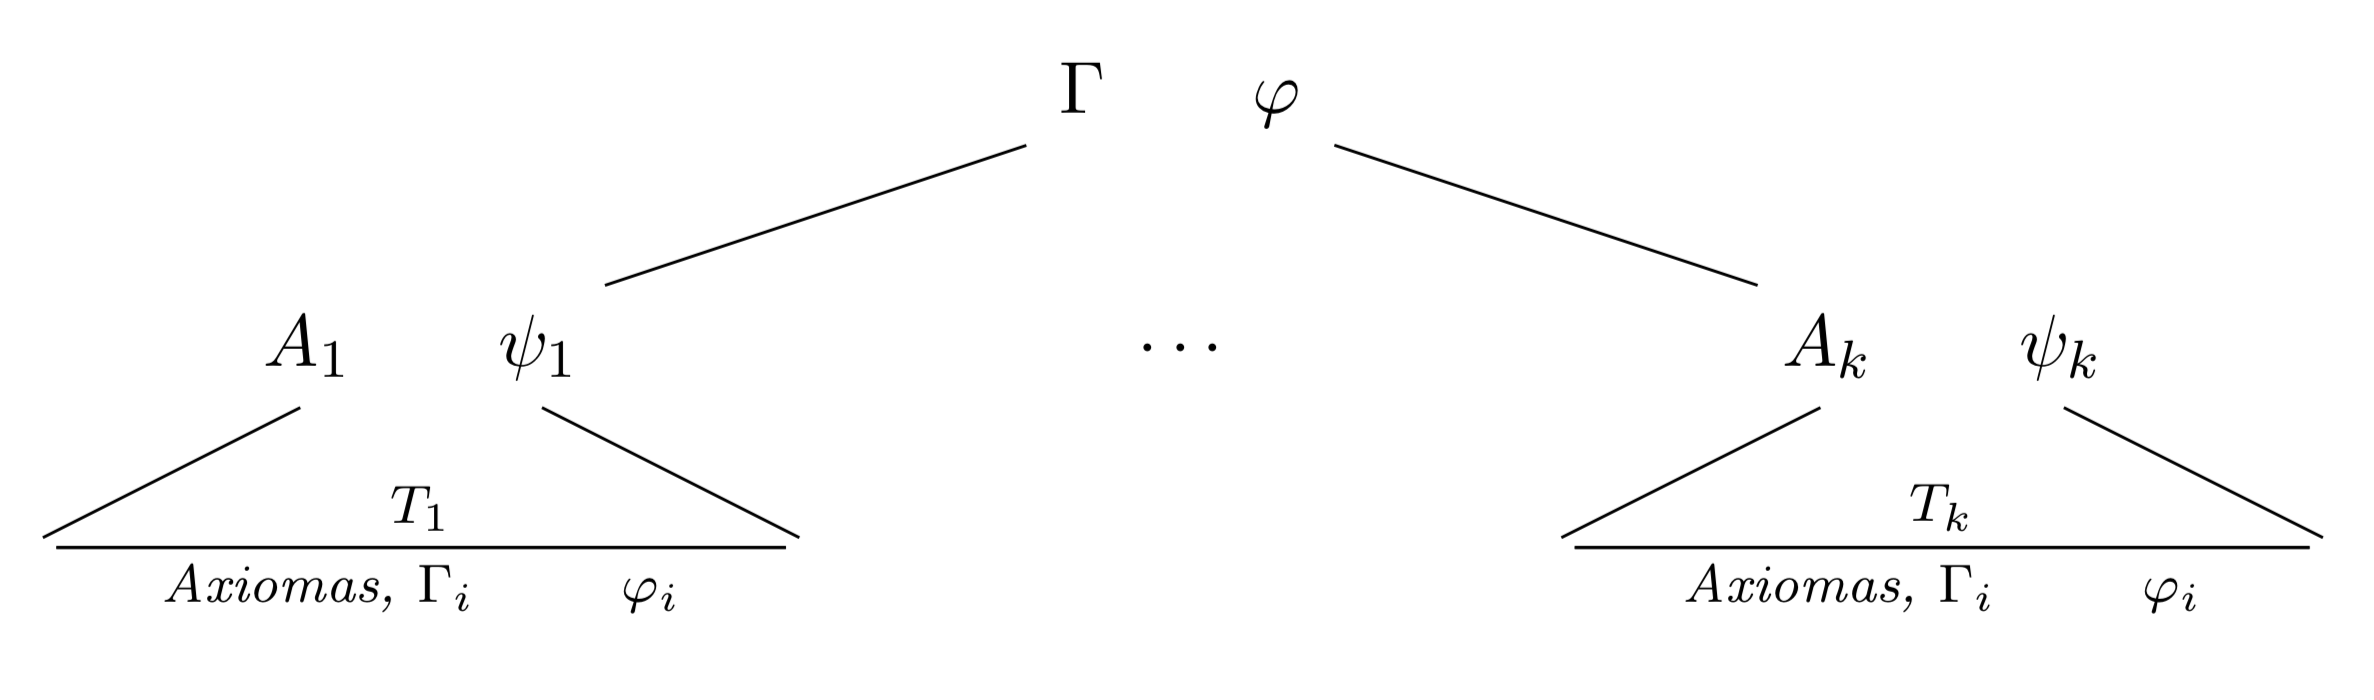
\includegraphics[scale = 0.3]{figures/arbol3.png}
\end{center}
\begin{comment}
% https://tikzcd.yichuanshen.de/#N4Igdg9gJgpgziAXAbVABwnAlgFyxMJZAZgBoAGAXVJADcBDAGwFcYkQAdDgcXoFs+9LgEdhzelC4MATmgAWWEAF9S6TLnyEUARlLbqdJq3YBBAPraRYiVzTYLy1SAzY8BImX00GLNok4cAMZQEDgIKmqumkQArHoGPsb+5gDWVuKSHHZYZimOkRruKOSkAEwJRn4g+c7qblrIpWUVvuw1LoUNACzN3pVtEbVRRcgAbL2Grf7KBjBQAObwRKAAZtIQfEglIDgQSGSTSWDMjIw0jPQARjCMAAp10f6MMCs4IDRyMBLskGBsg2sNlsaLskLpDn5jqdzlcbvdhloQM9Xu8QJ9vv5fv8nIDNohwaDED0IUgoWckbC7g8ikiXm8Pl8oD8CNjVus8QS9og4iTEGSYdcqQj2Mj6WjGcy-jVcfsQVzxrz+RTBfDOiK6aj0UzMSzpezZTsuQB2PpTJUXFXUxGizUSnVSgH6olypA8xJVAAqDgFcKt6pRDIx4F1jqBiAVhJNvJAXryPqFaqeGsD2uDDpxTp5hOJWslbFNSQCOBgAA88DhgCYS-hBHBSAACJRcXgCehmLDpGwcGTyHKKUN4qOEhW5+356NcYtl3CV6sbeh1xvN-iCdudzI9hTtmZKIA
\begin{tikzcd}
                              &                                                         &                                                                       & \Gamma\qquad\varphi \arrow[rrd, no head] \arrow[lld, no head] &                               &                                                         &                                                                       \\
                              & A_1\qquad\psi_1 \arrow[ld, no head] \arrow[rd, no head] &                                                                       & \cdots                                                        &                               & A_k\qquad\psi_k \arrow[ld, no head] \arrow[rd, no head] &                                                                       \\
{} \arrow[rr, "T_1", no head] &                                                         & {} \arrow[ll, "{\textit{Axiomas, }\Gamma_i\qquad\varphi_i}", no head] &                                                               & {} \arrow[rr, "T_k", no head] &                                                         & {} \arrow[ll, "{\textit{Axiomas, }\Gamma_i\qquad\varphi_i}", no head]
\end{tikzcd}

\end{comment}
donde 
\begin{prooftree}
\AxiomC{$A_1 \idash \psi_1$}
\AxiomC{$A_k \idash \psi_k$}
\BinaryInfC{$\Gamma \idash \varphi$}(R')
\end{prooftree}
es una regla correcta, y cada $A_l\idash\psi_l$ tiene un árbol de deducción $T_l$ de altura $<m$.\\

Como el árbol de deducción $T_l$ tiene altura $<m$, y tiene en la raíz a $A_l\idash\psi_l$ y en las hojas axiomas o elementos de $\{\Gamma_1\idash\varphi_1,\dots,\Gamma_n\idash\varphi_n\}$, por hipótesis de inducción tenemos que la regla

\begin{prooftree}
\AxiomC{$\Gamma_1 \idash \varphi_1$}
\AxiomC{$\Gamma_n \idash \varphi_n$}
\BinaryInfC{$A_l \idash \psi_l$}($R_l$)
\end{prooftree}
es correcta, para $l=1,\dots,k$.\\

De modo que si suponemos que $\Gamma_1 \idash \varphi_1,\dots,\Gamma_n \idash \varphi_n$ son correctas, entonces $A_l \idash \psi_l$ es correcta para $l=1,\dots,k$. Por tanto, como $\regla{R'}$ es correcta, $\Gamma \idash \varphi$ también es correcta. Por tanto $\regla{R}$ es correcta.
\end{itemize}
\end{proof}

\begin{cor}\label{derivcorr2}
Toda regla derivada es correcta.
\end{cor}
\begin{proof}
Directo usando \ref{bacorr} y \ref{derivcorr}.
\end{proof}
\begin{cor}\textit{(Corrección)} Si $\Phi\vdash\varphi$, entonces $\Phi\vDash\varphi$.
\end{cor}
\begin{proof}
Por definición, si $\Phi\vdash\varphi$, hay un subconjunto finito $\Gamma\subseteq\Phi$ tal que $\vdash\Gamma\idash\varphi$. Es decir, $\displaystyle\frac{}{\Gamma\idash\varphi}$ es un axioma derivado, y por \ref{derivcorr2} es correcto. De modo que se cumple $\Gamma\vDash\varphi$. Esto, a su vez, implica que $\Phi\vDash\varphi$.
\end{proof}

\section{Completitud}
Como en el caso de los \textit{tableaux} de primer orden, la completitud va a ser más complicada de demostrar que la corrección.

\begin{definition}
Decimos que un conjunto $\Phi$ es \textit{consistente}, $con(\Phi)$, si $\Phi\nvdash\bot$, es decir, no existe un subconjunto finito $\Gamma\subseteq\Phi$ tal que $\vdash\Gamma\idash\bot$.
\end{definition}

El resultado que nos llevará la gran mayoría de la sección será demostrar el teorema \ref{corsat}, que dice que si un conjunto $\Phi$ es consistente, entonces es satisfactible. Una vez demostrado este teorema, la completitud se deducirá sin mucho esfuerzo. Comenzamos con el siguiente lema:

\begin{lema}\label{regder}
Las siguientes reglas son derivadas:
\begin{enumerate}
    \item Si $\alpha$ es $\alpha$-fórmula, $$(\alpha) \frac{\Gamma, \alpha_1, \alpha_2, \alpha \idash \chi}{\Gamma, \alpha \qquad \chi}$$
    \item Si $\beta$ es $\beta$-fórmula, $$(\beta)\frac{\Gamma, \beta_1, \beta \idash \chi \quad\quad \Gamma, \beta_2, \beta \idash \chi}{\Gamma, \beta \idash \chi}$$
    \item Si $\sigma$ es $\sigma$-fórmula, $$(\sigma)\frac{\Gamma, \sigma, \sigma_1 \idash \chi}{\Gamma, \sigma \idash \chi}$$
    \item SI $\gamma$ es $\gamma$-fórmula y $t\in TERM_S$ $$(\gamma)\frac{\Gamma, \gamma(t), \gamma \idash \chi}{\Gamma, \gamma \idash \chi}$$
    \item Si $\delta$ es $\delta$-fórmula y $c\in C_A$ es nueva, $$(\delta)\frac{\Gamma, \delta(c), \delta \idash \chi}{\Gamma, \delta \idash \chi}$$
    \item Si $\theta \in EQ_S$ es $\theta$-fórmula, $$(\theta)\frac{\Gamma, \theta \idash \chi}{\Gamma \idash \chi}$$
\end{enumerate}
\end{lema}

\begin{proof} No se incluye. En cada apartado es necesario dividir en casos y crear árboles de deducción para cada caso.
\begin{comment}
No se va a hacer explícitamente. Requiere crear árboles de deducción para todas estas reglas. En los apartados 1 y 2, dada la definición  por casos de las reglas $\alpha$ y $\beta$, esto requiere 3 árboles en cada apartado. De igual forma hacen falta 3 árboles en el apartado 3, y 2 árboles en los apartados 4 y 5. El apartado 6 se divide en más casos y el caso de los axiomas $(ST_1)$ y $(ST_2)$ es más complicado y requiere argumentos inducción y la ley de sustitución generalizada.
\end{comment}
\end{proof}


\begin{prop}\label{condramas}
Sea $T$ tableau finito para $\Phi$. Sean:
$$\Gamma := \{\varphi \in \Phi \, \, | \, \, \varphi \text{ aparece en } T\}$$
$$\Gamma_r:= \{\varphi \,\, | \,\, \varphi \text{ aparece en la rama } r\}$$
Si para toda rama $r$ de $T$ se cumple que, dada la fórmula $\chi$, $\vdash \Gamma_r \idash \chi$, entonces $\vdash \Gamma \idash \chi$. 
\end{prop}
\begin{proof}
Sea $T$ \textit{tableau} finito para $\Phi$. Entonces se puede construir en un número finito de pasos $T_0, \dots, T_n$ mediante la aplicación de las reglas $R_1, \dots, R_n$.

Realizamos la demostración por inducción sobre $n$. Denotamos $\Gamma_k :=  \{\varphi \in \Phi \, \, | \, \, \varphi \text{ aparece en } T_k\}$.

Si $n = 0$ entonces tenemos un \textit{tableaux} inicial $T_0 =$
\begin{tikzcd}
\varphi_1 \arrow[d, no head]          \\
\varphi_2 \arrow[dd, no head, dotted] \\
                                      \\
\varphi_k                            
\end{tikzcd}, con $\{\varphi_1, \dots, \varphi_k\} \subseteq \Phi$. Por tanto, solo tenemos una rama $r$ que además verifica que $\Gamma = \Gamma_r$, de lo que se sigue el resultado.

Sea $n\geq 1$, supongamos que el resultado se cumple para $T_{n-1}$. Para ver que se cumple en $T_n$, tenemos que distinguir casos dependiendo de la regla que sea $R_n$. En todos los casos, usaremos la letra $r$ para nombrar las ramas de $T_{n-1}$ y $s$ para nombrar a las ramas de $T_n$.
\begin{itemize}
    \item Si $R_n = R_{\alpha}$, entonces en $T_{n-1}$ tenemos una rama $r_0$ conteniendo la $\alpha$-fórmula $\alpha$, y esa rama se extiende añadiendo $\alpha_1$ y $\alpha_2$ para formar la rama $s_0$ de $T_n$. \\
    
    Supongamos ahora que $\vdash\Gamma_s\idash\chi$ para toda rama $s$ de $T_{n}$ y queremos llegar a que se cumple $\vdash\Gamma_n\idash\chi$. Veamos primero que para toda rama $r$ en $T_{n-1}$, tenemos $\vdash\Gamma_r\idash\chi$. Para ello basta comprobar que $\vdash\Gamma_{r_0}\idash\chi$, ya que el resto de ramas $r$ que no son $r_0$ no se han extendido y son también ramas de $T_n$.\\
    
    Pero sabemos que $\vdash\Gamma_{s_0}\idash\chi$. Además, como $\alpha\in\Gamma_{r_0}$ y $\Gamma_{s_0}=\Gamma_{r_0}\cup\{\alpha_1,\alpha_2\}$, por el apartado 1 de \ref{regder} la regla $\frac{\Gamma_{s_0}\idash\chi}{\Gamma_{r_0}\idash\chi}$ es derivada. Por tanto como se cumple $\vdash\Gamma_{s_0}\idash\chi$, también se cumple $\vdash\Gamma_{r_0}\idash\chi$.\\
    
    Como tenemos $\vdash\Gamma_r\idash\chi$ para toda rama $r$ de $T_{n-1},$ por hipótesis de inducción $\vdash\Gamma_{n-1}\idash\chi$. Como $\Gamma_{n-1}\subseteq\Gamma_n$, esto implica $\vdash\Gamma_n\idash\chi$.\\
    
    \item Si $R_n = R_{\beta}$, entonces en $T_{n-1}$ tenemos una rama $r_0$ conteniendo la $\beta$-fórmula $\beta$, y esa misma rama se extiende añadiendo $\beta_1$ y $\beta_2$ para formar las ramas $s_1$ y $s_2$ de $T_n$, respectivamente. \\
    
    Supongamos ahora que $\vdash\Gamma_s\idash\chi$ para toda rama $s$ de $T_{n}$ y queremos llegar a que se cumple $\vdash\Gamma_n\idash\chi$. Veamos primero que para toda rama $r$ en $T_{n-1}$, tenemos $\vdash\Gamma_r\idash\chi$. Para ello basta comprobar que $\vdash\Gamma_{r_0}\idash\chi$, ya que el resto de ramas $r$ que no son $r_0$ no se han extendido y son también ramas de $T_n$.\\
    
    Pero sabemos que $\vdash\Gamma_{s_1}\idash\chi$ y $\vdash\Gamma_{s_2}\idash\chi$. Además, como $\beta\in\Gamma_{r_0}$ y $\Gamma_{s_1}=\Gamma_{r_0}\cup\{\beta_1\}$, $\Gamma_{s_2}=\Gamma_{r_0}\cup\{\beta_2\}$ por el apartado 2 de \ref{regder} la regla $\frac{\Gamma_{s_1}\idash\chi\qquad \Gamma_{s_2}\idash\chi}{\Gamma_{r_0}\idash\chi}$ es derivada. Por tanto como se cumplen $\vdash\Gamma_{s_1}\idash\chi$ y $\vdash\Gamma_{s_2}\idash\chi$, también se cumple $\vdash\Gamma_{r_0}\idash\chi$.\\
    
    Como tenemos $\vdash\Gamma_r\idash\chi$ para toda rama $r$ de $T_{n-1},$ por hipótesis de inducción $\vdash\Gamma_{n-1}\idash\chi$. Como $\Gamma_{n-1}\subseteq\Gamma_n$, esto implica $\vdash\Gamma_n\idash\chi$.\\



    \item Si $R_n = R_{\sigma}$, entonces en $T_{n-1}$ tenemos una rama $r_0$ conteniendo la $\sigma$-fórmula $\sigma$, y esa misma rama se extiende añadiendo $\sigma_1$ para formar la rama $s_0$ de $T_n$. \\
    
    Supongamos ahora que $\vdash\Gamma_s\idash\chi$ para toda rama $s$ de $T_{n}$ y queremos llegar a que se cumple $\vdash\Gamma_n\idash\chi$. Veamos primero que para toda rama $r$ en $T_{n-1}$, tenemos $\vdash\Gamma_r\idash\chi$. Para ello basta comprobar que $\vdash\Gamma_{r_0}\idash\chi$, ya que el resto de ramas $r$ que no son $r_0$ no se han extendido y son también ramas de $T_n$.\\
    
    Pero sabemos que $\vdash\Gamma_{s_0}\idash\chi$. Además, como $\sigma\in\Gamma_{r_0}$ y $\Gamma_{s_0}=\Gamma_{r_0}\cup\{\sigma_1\}$, por el apartado 3 de \ref{regder} la regla $\frac{\Gamma_{s_0}\idash\chi}{\Gamma_{r_0}\idash\chi}$ es derivada. Por tanto como se cumple $\vdash\Gamma_{s_0}\idash\chi$, también se cumple $\vdash\Gamma_{r_0}\idash\chi$.\\
    
    Como tenemos $\vdash\Gamma_r\idash\chi$ para toda rama $r$ de $T_{n-1},$ por hipótesis de inducción $\vdash\Gamma_{n-1}\idash\chi$. Como $\Gamma_{n-1}\subseteq\Gamma_n$, esto implica $\vdash\Gamma_n\idash\chi$.\\
    
    \item Las reglas $\gamma,\delta$ siguen el mismo razonamiento que la $\sigma$ cambiando $\sigma$ por $\gamma/\delta$ y $\sigma_1$ por $\gamma(t)/\delta(c)$ respectivamente, y usando los apartados $4/5$ de \ref{regder}.

    La regla $\theta$ también se hace de forma similar, viendo que si en la regla añadimos una fórmula $\theta$ a una rama $r_0$ de $T_{n-1}$ para obtener una rama $s_0$ de $T_n$, entonces por el apartado 6 de \ref{regder}, la regla $\frac{\Gamma_{s_0}\idash\chi}{\Gamma_{r_0}\idash\chi}$ es derivada.

    \item Si $R_n=R_{hip}$, entonces en $T_{n-1}$ tenemos una rama $r_0$, a la que añadimos la fórmula $\varphi$ de $\Phi$ para  formar la rama $s_0$ de $T_n$. \\
    
    Supongamos ahora que $\vdash\Gamma_s\idash\chi$ para toda rama $s$ de $T_{n}$ y queremos llegar a que se cumple $\vdash\Gamma_n\idash\chi$. Veamos primero que para toda rama $r$ en $T_{n-1}$, tenemos $\vdash \Gamma_r\idash \varphi\to\chi$. Dos  casos:
    \begin{itemize}
        \item $r\neq r_0$. Entonces  $r$ también es una rama de $T_n$, por tanto sabemos $\vdash\Gamma_r\idash\chi$. Por $(\mathbf{FS})$, obtenemos $\vdash\Gamma_r,\varphi\idash\chi$, y por $(\to\mathbf{C})$, llegamos a que $\vdash\Gamma_r\idash\varphi\to\chi$.
        \item $r=r_0$. Sabemos que $\vdash\Gamma_{s_0}\idash\chi$, por tanto por $(\to\mathbf{C})$, tenemos que $\vdash\Gamma_{s_0}\setminus\{\varphi\}\idash\varphi\to\chi$. Como $\Gamma_{s_0}\setminus\{\varphi\}\subseteq\Gamma_{r_0}$, por $(\mathbf{FS})$ tenemos que $\vdash\Gamma_{r_0}\idash\varphi\to\chi$.
    \end{itemize}
    De modo que como tenemos que $\vdash \Gamma_r\idash \varphi\to\chi$ para toda rama $r$ de  $T_{n-1}$, por hipótesis de inducción con la fórmula $\varphi\to\chi$ tenemos que $\vdash \Gamma_{n-1}\idash \varphi\to\chi$. Como $\Gamma_{n-1}\subseteq\Gamma_n$, tenemos $\vdash \Gamma_n\idash \varphi\to\chi$. Como además $\vdash \Gamma_n\idash \varphi$ es un axioma del supuesto, por $(\textbf{MP})$ deducimos que $\vdash \Gamma_n\idash \chi$, como queríamos.



    

\end{itemize}
\end{proof}

\begin{cor}
Si el conjunto de fórmulas $\Phi$ tiene un tableau cerrado, entonces $\Phi \vdash \bot$.
\end{cor}
\begin{proof}
Sea $T$ un \textit{tableau} cerrado para $\Phi$. Sea $r$ rama de $T$. Si $\bot \in \Gamma_r$, entonces $\vdash \Gamma_r \idash \bot$, por $\mathbf{(SP)}$. Si existe cierta $\varphi$ tal que $\varphi, \neg\varphi\in \Gamma_r$, entonces, por $\mathbf{(CT_2)}$, $\vdash \Gamma_r \idash \bot$. 

De modo que como para cada rama $r$ se cumple $\vdash \Gamma_r \idash \bot$, por \ref{condramas} tenemos $\vdash \Gamma \idash \bot$, con $\Gamma := \{\varphi\in \Phi \, \, | \, \, \varphi \text{ está en } T\}$. Como $\Gamma$ es subconjunto finito de $\Phi$, $\Phi \vdash \bot$.
\end{proof}



\begin{theorem}\label{corsat}
Si $con(\Phi)$, entonces $Sat(\Phi)$.
\end{theorem}
\begin{proof}
Es la forma contrarrecíproca del resultado anterior.
\end{proof}

\begin{cor}(Completitud)
Si $\Phi \vDash \varphi$, entonces $\Phi \vdash \varphi$.
\end{cor}
\begin{proof}
Si $\Phi \vDash \varphi$ entonces $Insat(\Phi \cup \{\neg \varphi\})$, es decir, por \ref{corsat} es falso que $con(\Phi\cup \{\neg \varphi\})$, y entonces existe un subconjunto finito $\Gamma\subseteq\Phi\cup \{\neg \varphi\}$ tal que $\vdash\Gamma\idash\bot$.
Tenemos, por tanto, 
\begin{center}
    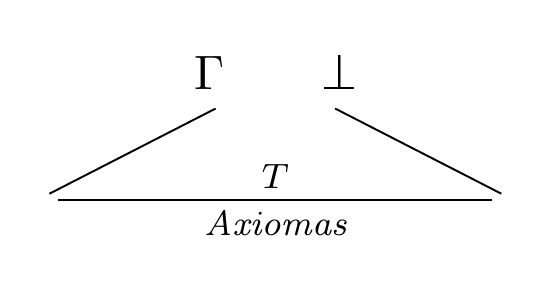
\includegraphics[scale = 0.3]{figures/arbol4.png}
\end{center}
Veamos si existe un subconjunto finito $\Delta \subseteq \Phi$ tal que $\vdash\Delta\idash\varphi$.
\begin{itemize}
    \item Si $\neg \varphi \notin \Gamma$, tomando $\Delta := \Gamma$ obtenemos:
\begin{center}
    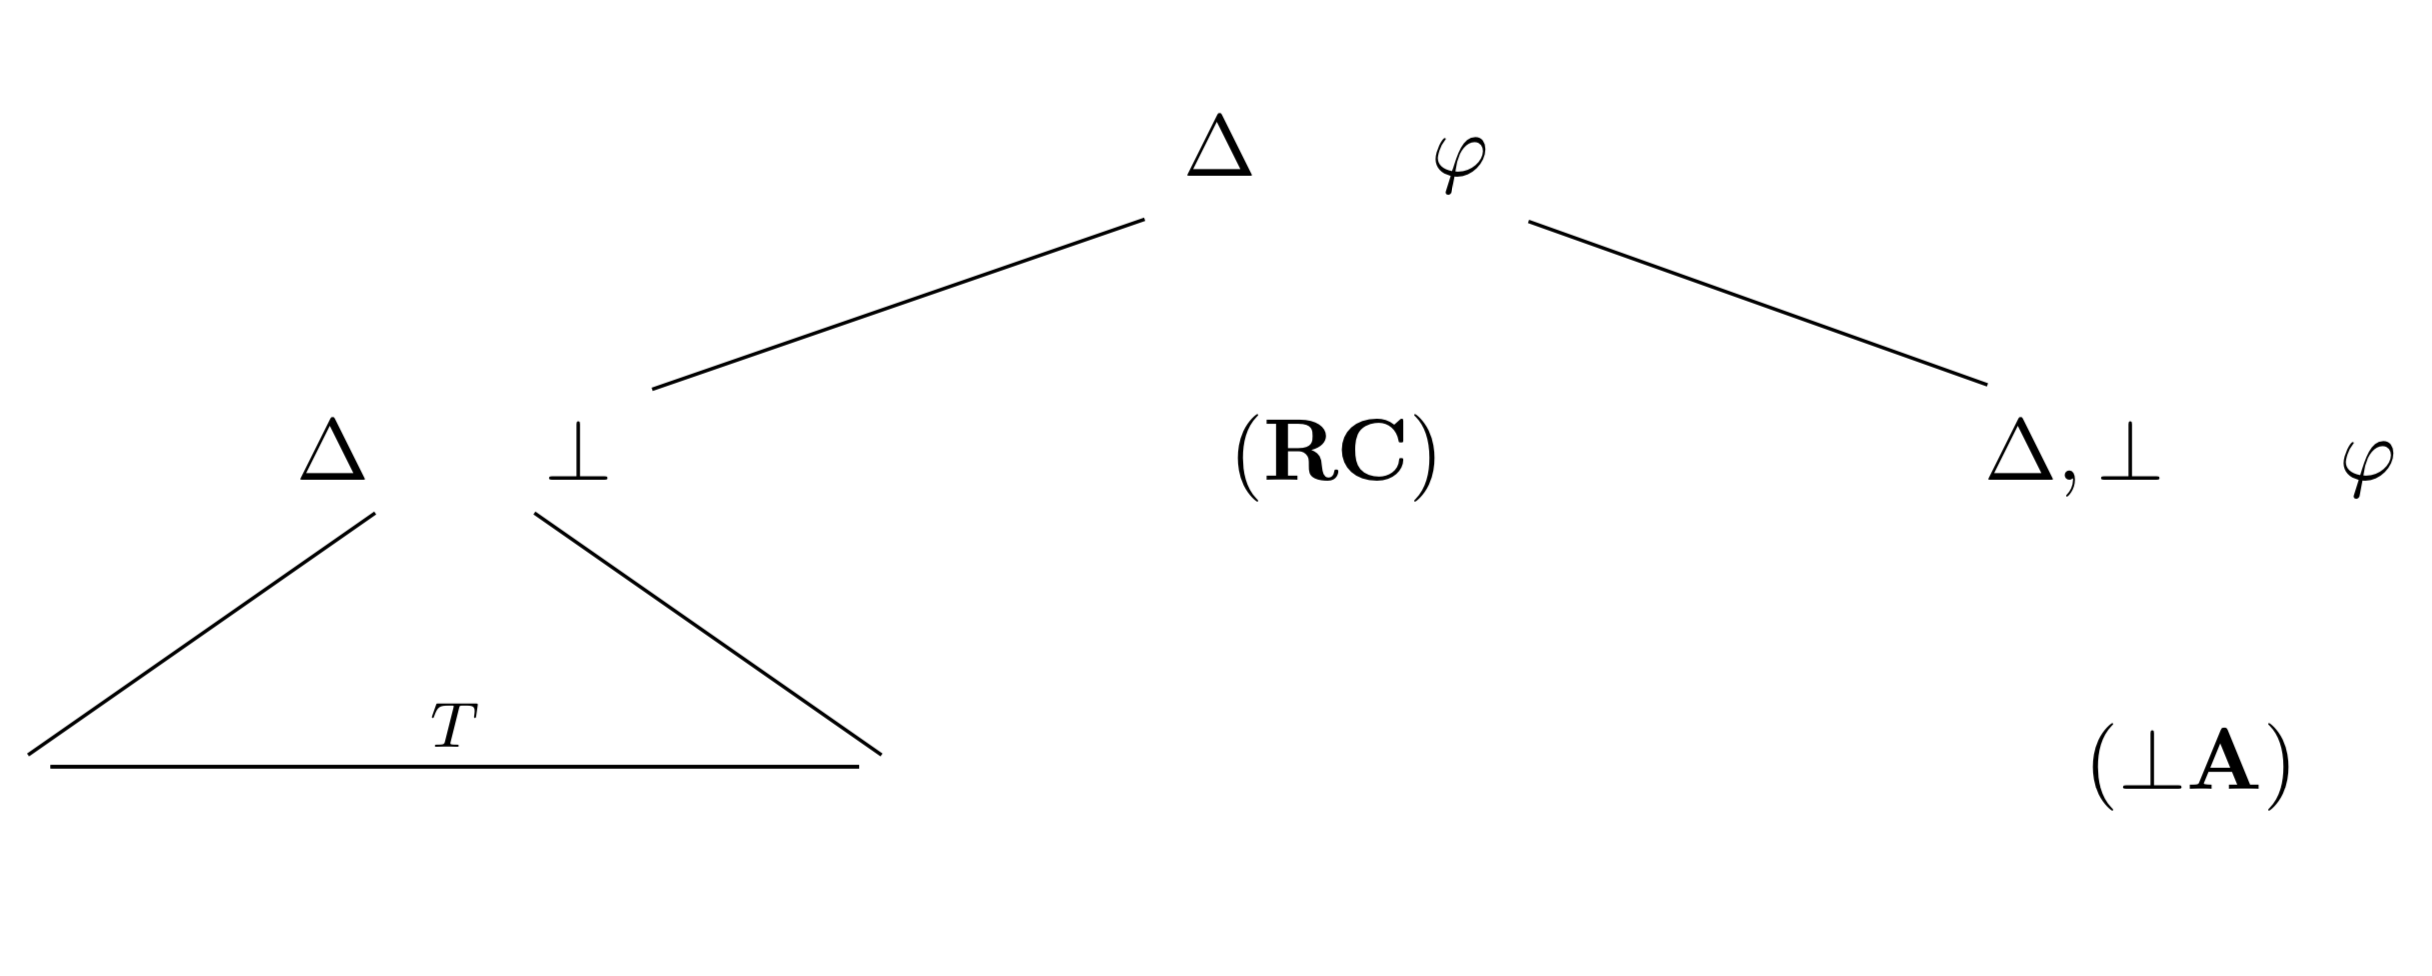
\includegraphics[scale = 0.23]{figures/arbol5.png}
\end{center}
\begin{comment}
% https://tikzcd.yichuanshen.de/#N4Igdg9gJgpgziAXAbVABwnAlgFyxMJZAZgBoAGAXVJADcBDAGwFcYkQAdDgcXoFs+9LgEdhzelC4MATmgAWWEAF9S6TLnyEUARlLbqdJq3ZdeA+gAIRYiVY4AjCDmWqQGbHgJEy+mgxZsiCAAFFw4MAAeOPYAZsAASgDCSgCULmoemkQArHoG-sZBpvyCpHaOOHai4lB2MvKKKhkaXijkpABM+UaBIOlu6p5ayB2d3QHs-e4tw7ldfj3soQ5OXII4crHAAIKpygYwUADm8ESgMdIQfEjtIDgQSGSGE4hgzIyMNIz09jCMAAqDLJBRgwGLOGhyGASdiQMBsJogC5XG40e5IXTPQpvD5fH5-QGZVogUHgkCQ6FQWEEBGuZHXRCY9GIAAsCxeOM+JPxAKBxNJEJAUJhQThtPOlwZTIeiFyWMCnLxv15RK0JLBguFVNFNP69KQbLuMrlBV6ABVydzlYSZuwBZatdT4XrJUg5czDaakIqrQS+Wr7RSReBdUpKEogA
\begin{tikzcd}
                            &                                                            &                        & \Gamma\qquad\varphi \arrow[rrd, no head] \arrow[lld, no head] &  &                               \\
                            & \Gamma \qquad \bot \arrow[ld, no head] \arrow[rd, no head] &                        & (\textbf{RC})                                                 &  & {\Gamma, \bot \qquad \varphi} \\
{} \arrow[rr, "T", no head] &                                                            & {} \arrow[ll, no head] &                                                               &  & (\bot\mathbf{A})             
\end{tikzcd}
\end{comment}

    \item Si $\neg \varphi \in \Delta$, tomando $\Delta := \Gamma \setminus \{\neg \varphi\}$ obtenemos:
\begin{center}
    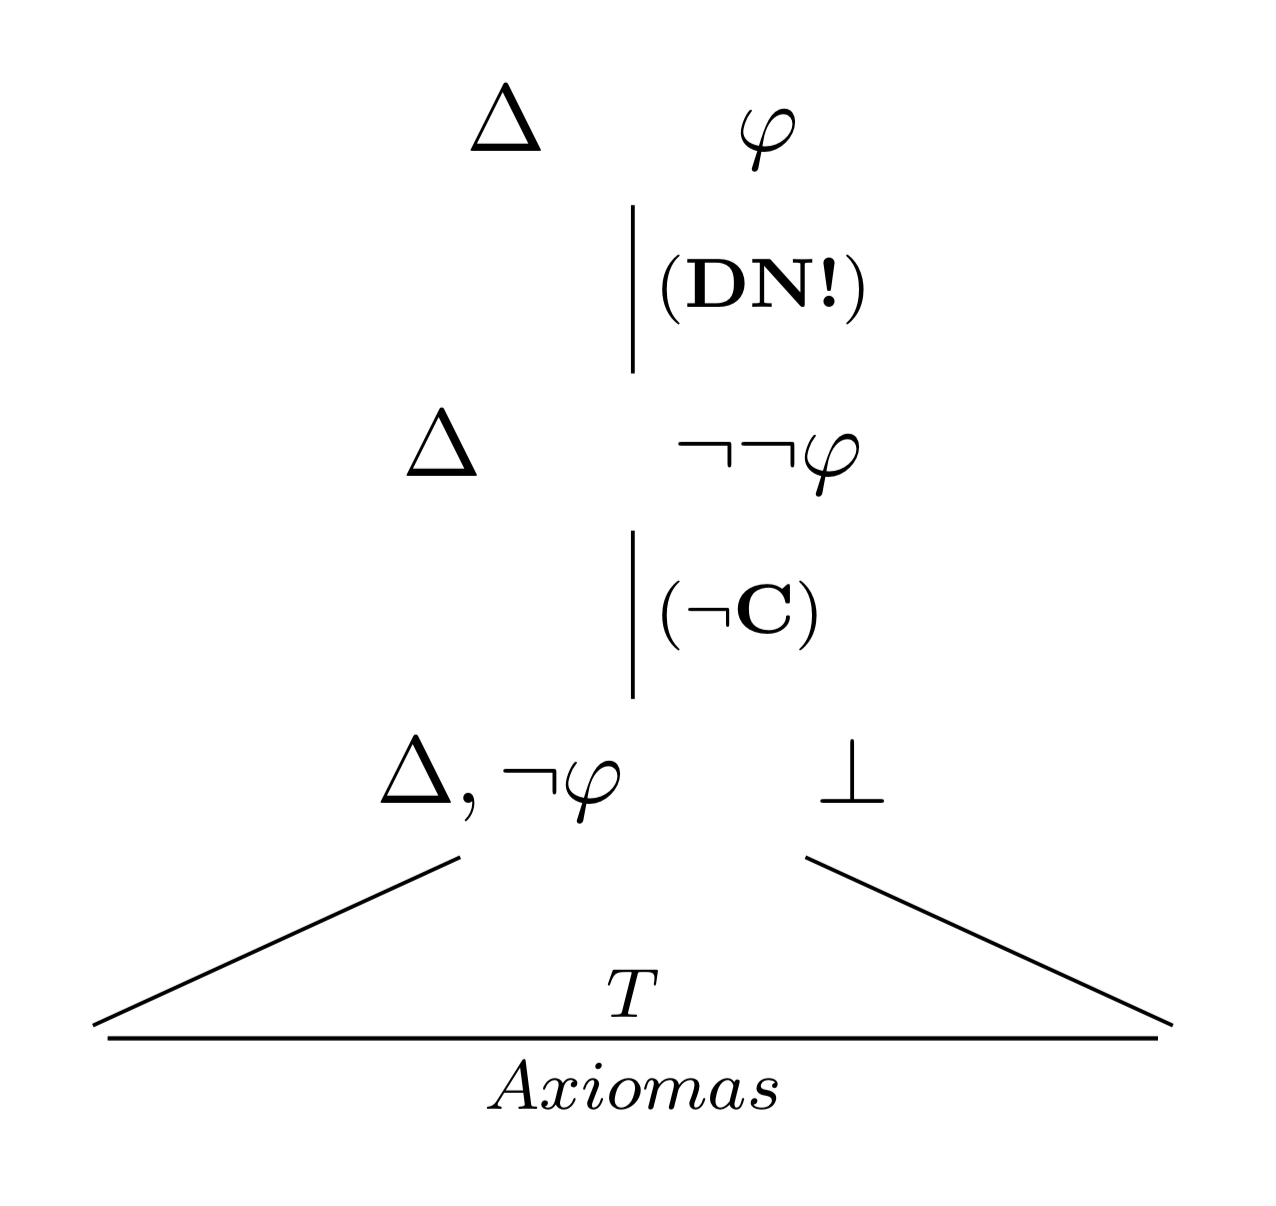
\includegraphics[scale = 0.23]{figures/arbol6.png}
\end{center} 
\begin{comment}
% https://tikzcd.yichuanshen.de/#N4Igdg9gJgpgziAXAbVABwnAlgFyxMJZARgBoAmAXVJADcBDAGwFcYkQAdDgERkZ3qkABFzAwA5lwYAnNAAssXAI5Lm9KFwBGEHCAC+pdJlz5CKAAykAzNTpNW7fYZAZseAkXLXbDFm0QgTkZupkRkxD72-pw8fAIiHCpqUAlikhxpUvSyCkEuxu5mJKTmkX7sXLz89AlJ6gky8lhC+rYwUOLwRKAAZtIQALZIliA4EEhkduWIYMyMjDSM9Jp8AAoFoQGMMD26NHIw6uyQYnl9g8M0Y0heUw4zcwsgSyuM6yEeWzt7IAdHASc2AZev0hohJtdELdfPcQAAVECLZZrDafZ7fRG-Q5QY4EIHOc5g26QyZ-HEAvGYmHRACCAA98AN6AhgSBCZdRuNEFZ9tjcacka93iY0dIsOI5D9qewABSiCRcHAwOk4TQ9YAAYT0AEozqCkDzOUgACy8-7gSmClEfMwgMUSqVRWWK5Wq9XcAByAEIda09EA
\begin{tikzcd}
                            & \Delta \qquad \varphi                                                                                           &                                   \\
                            & \Delta \qquad \neg\neg\varphi \arrow[u, "(\textbf{DN!})"', no head]                                             &                                   \\
                            & {\Delta, \neg\varphi\qquad\bot} \arrow[ld, no head] \arrow[rd, no head] \arrow[u, "(\neg\textbf{C})"', no head] &                                   \\
{} \arrow[rr, "T", no head] &                                                                                                                 & {} \arrow[ll, "Axiomas", no head]
\end{tikzcd}
\end{comment}
\end{itemize}
de modo que en ambos casos se cumple el enunciado.
\end{proof}

De modo que hemos visto que si $S$ es signatura numerable y $\Phi \subseteq FORM_S$ es insatisfactible, entonces $\Phi$ tiene \textit{tableau} cerrado y es, por tanto, inconsistente. De hecho, este resultado también se puede demostrar cuando $S$ no es numerable.\footnote{Este resultado se puede encontrar en el capítulo 5 del libro \textit{Mathematical Logic}, de los autores H.-D. Ebbinghaus, J. Flum y W. Thomas.}\\


Finalmente, demos una visión global de lo que hemos estudiado en estas últimas subsecciones. Partiendo de los dos pares de conceptos \textit{deducción formal}-\textit{consistencia}  y \textit{corrección}-\textit{satisfactibilidad} hemos establecido un nexo entre las perspectivas sintáctica y semántica, respectivamente representadas por cada par de tales conceptos. \\

Este nexo consiste en los Teoremas de Corrección y Completitud, que nos permiten pasar `de un lado a otro': El teorema de corrección nos permite traducir algunas afirmaciones sintácticas a semánticas, y el de completitud nos permite traducir afirmaciones semánticas a sintácticas.\\

A continuación mostramos la correspondencia que hemos definido:
\begin{align*}
    \text{\large Sintaxis} & \qquad  \text{\large Semántica} \\   
    \text{Fórmulas} & \Longleftrightarrow  \text{ Modelos} \\
    \Phi \vdash \varphi \quad (\Phi \vdash_{tb} \varphi) & \Longleftrightarrow  \Phi \vDash \varphi \\
    con(\Phi) & \Longleftrightarrow sat(\Phi) \\
    \vdash \varphi \leftrightarrow \psi & \Longleftrightarrow \varphi \sim \psi \\
    \vdash \varphi & \Longleftrightarrow \vDash \varphi
\end{align*}
